\documentclass[12pt, a4paper]{article}

% ── Encoding & Sprache ───────────────────────────────────────
\usepackage[T1]{fontenc}
\usepackage[utf8]{inputenc}
\usepackage[german]{babel}
\usepackage{microtype}

% ── Seitenlayout ─────────────────────────────────────────────
\usepackage{geometry}
\geometry{margin=2.5cm}

% ── Mathematik ───────────────────────────────────────────────
\usepackage{amsmath, amssymb, amsthm, mathtools}
\usepackage{bm}

% ── Grafik & Tabellen ────────────────────────────────────────
\usepackage{graphicx}
\usepackage{float}
\usepackage{caption}
\usepackage{subcaption}
\usepackage{booktabs}
\usepackage{array}
\usepackage{multirow}
\usepackage[table]{xcolor}

% ── Referenzen & Links ───────────────────────────────────────
\usepackage{hyperref}
\usepackage[german]{cleveref}
\usepackage{url}

% ── Listen & Aufzählungen ────────────────────────────────────
\usepackage{enumitem}
\setlist[itemize,1]{label=--}

% ── Layout-Pakete ────────────────────────────────────────────
\usepackage{setspace}
\usepackage{fancyhdr}
\usepackage{titlesec}
\usepackage{abstract}
\usepackage{tikz}
\usetikzlibrary{arrows.meta, positioning, shapes.geometric}

% ── Code-Listings ────────────────────────────────────────────
\usepackage{listings}

% ── Farben ──────────────────────────────────────────────────
\definecolor{BlauDunkel}{HTML}{1414B8}
\definecolor{RotDunkel} {HTML}{8B1A1A}
\definecolor{GruenDunkel}{HTML}{1A5C2A}
\definecolor{OrangeDunkel}{HTML}{C45C00}
\definecolor{LilaFarbe}{HTML}{4B0082}
\definecolor{GrauHell}  {HTML}{F2F2EF}
\definecolor{GrauMittel}{HTML}{808080}
\definecolor{mainblue}  {RGB}{25, 70, 140}
\definecolor{accentred} {RGB}{180, 50, 30}
\definecolor{lightgray} {RGB}{245, 245, 248}
\definecolor{darkgray}  {RGB}{60, 60, 70}

% ── Hyperref ─────────────────────────────────────────────────
\hypersetup{
  colorlinks = true,
  linkcolor  = BlauDunkel,
  citecolor  = RotDunkel,
  urlcolor   = LilaFarbe,
  pdftitle   = {GSKA-N Framework: Krebsausbruch, Prädisposition, Stress und biologische Netzwerke},
  pdfauthor  = {Stephan Epp},
  pdfsubject = {Mathematische Krebsmodellierung}
}

% ── Theorem-Umgebungen ───────────────────────────────────────
\theoremstyle{definition}
\newtheorem{definition}{Definition}[section]
\newtheorem{satz}[definition]{Satz}
\newtheorem{lemma}[definition]{Lemma}
\newtheorem{korollar}[definition]{Korollar}
\newtheorem{proposition}[definition]{Proposition}
\newtheorem{annahme}[definition]{Annahme}
\newtheorem{beispiel}[definition]{Beispiel}
\newtheorem{bemerkung}[definition]{Bemerkung}
\theoremstyle{remark}
\newtheorem*{beweis*}{Beweis}

% ── Code-Stil ────────────────────────────────────────────────
\lstset{
  basicstyle   = \ttfamily\footnotesize,
  keywordstyle = \color{mainblue}\bfseries,
  commentstyle = \color{GrauMittel}\itshape,
  stringstyle  = \color{accentred},
  numbers      = left,
  numberstyle  = \tiny\color{GrauMittel},
  breaklines   = true,
  frame        = single,
  rulecolor    = \color{GrauMittel},
  backgroundcolor = \color{lightgray},
  tabsize      = 4
}

% ── Eigene Operatoren & Makros ───────────────────────────────
\DeclareMathOperator{\logit}{logit}
\DeclareMathOperator{\sigmoid}{\sigma}
\newcommand{\R}{\mathbb{R}}
\newcommand{\N}{\mathbb{N}}
\newcommand{\E}{\mathbb{E}}
\newcommand{\Prob}{\mathbb{P}}
\newcommand{\calD}{\mathcal{D}}
\newcommand{\calG}{\mathcal{G}}
\newcommand{\calS}{\mathcal{S}}
\newcommand{\calN}{\mathcal{N}}
\newcommand{\calM}{\mathcal{M}}
\newcommand{\calA}{\mathcal{A}}
\newcommand{\subgraphalg}{\mathtt{SubgraphCheck}}
\newcommand{\rot}{\mathrm{rot}}
\newcommand{\LCS}{\mathrm{LCS}}
\newcommand{\sig}{\boldsymbol{\sigma}}
\newcommand{\GN}{G_{\calN}}


\title{\bfseries Genetische Prädisposition, Stressbelastung und biologische
    Netzwerke als interagierende Determinanten des Krebsausbruchs}
\date{27. April 2026}
\author{Stephan Epp}


\begin{document}

\maketitle
\tableofcontents
\newpage


%  TEIL I – DAS GSKA-MODELL


\part{Das GSKA-Modell}
\label{part:gska}


\section{Einleitung}
\label{sec:einleitung}

Die vorliegende Arbeit entwickelt das \emph{GSKA-N Framework} —
ein zweistufiges mathematisches Modell des Krebsausbruchs, das von
der molekularen Netzwerkebene bis zur klinischen Risikoschätzung reicht.

\textbf{Teil~I} definiert das \emph{Genetisch-Stochastische Krebsausbruch-Modell}
(GSKA): Die Ausbruchswahrscheinlichkeit $P(G,S) = \sigma(\alpha G + \beta S
+ \gamma GS - \theta)$ hängt von der genetischen Prädisposition $G \in [0,1]$
und der Stressbelastung $S \in [0,1]$ ab. Es werden Monotonieeigenschaften,
Iso-Wahrscheinlichkeits-Kurven, das Kompensationstheorem (hohe Prädisposition
kann durch günstige Umwelt kompensiert werden und umgekehrt) sowie eine
vollständige Phasenraumanalyse formal bewiesen.

\textbf{Teil~II} beantwortet die Frage, woher $G$ kommt: Der
\emph{Subgraph Algorithmus} (Epp 2026) erkennt krebsassoziierte
Netzwerkmotive ($M_1$: Feedback-Loop, $M_2$: Feed-Forward-Loop,
$M_3$: Hyper-Konnektivität) in einem Genregulationsnetzwerk $\calN$
mittels zyklischer Rotation und Signatur-Vergleich in optimaler $O(n^3)$-Zeit.
Die gewichtete Summe detektierter Motive definiert die
\emph{netzwerk-induzierte Prädisposition} $\GN \in [0,1]$,
die als $G$-Eingabe in das GSKA-Modell fließt.
Das resultierende \emph{N-GSKA-Modell} $P_\calN(S) = P(\GN, S)$
ist biologisch konsistent, monoton in der Kantenmenge und erlaubt
das \emph{Netzwerk-Kompensationstheorem}: gezielte Kantenstreichung
(z.\,B.\ durch Kinase-Inhibitoren) senkt $\GN$ und hebt die
kritische Stressschwelle an. Eine Monte-Carlo-Simulation
($N=200$ synthetische Netzwerke) validiert das Modell empirisch.

Die Frage, unter welchen Bedingungen Krebs ausbricht, gehört zu den zentralen
Problemen der modernen biomedizinischen Forschung. Epidemiologische Studien
belegen konsistent, dass zwei Klassen von Faktoren entscheidend sind:
einerseits die \emph{genetische Prädisposition} eines Individuums, quantifizierbar
durch Keimbahnmutationen, epigenetische Dispositionen und familiäre Häufungen,
und andererseits \emph{Umwelt- und Stressfaktoren}, die über oxidativen Stress,
chronische Entzündung, Immunsuppression und direkte Mutagene wirken.

Ein empirisch gut dokumentiertes, theoretisch jedoch unzureichend formalisiertes
Phänomen ist die \emph{kompensatorische Wechselwirkung}: Individuen mit hoher
genetischer Belastung erkranken in günstigen Lebensverhältnissen häufig nicht;
umgekehrt können Individuen mit geringer Prädisposition unter dauerhaftem Stress
dennoch erkranken. Diese Beobachtung verdient eine präzise mathematische Behandlung.

Das vorliegende Gesamtwerk leistet dies in zwei aufeinander aufbauenden Teilen.
\textbf{Teil~I} (\Cref{part:gska}) entwickelt das \emph{GSKA-Modell}, das die
Ausbruchswahrscheinlichkeit als sigmoide Funktion $P(G,S)$ formalisiert.
\textbf{Teil~II} (\Cref{part:bio}) legt mit dem \emph{Subgraph Algorithmus}
(Epp 2026, \cite{epp2026sub}) den molekularen Ursprung von $G$ offen: Die
Topologie des Genregulationsnetzwerks bestimmt über erkannte Netzwerkmotive
direkt die netzwerk-induzierte Prädisposition $\GN$.

\subsection{Beiträge dieser Arbeit}

\begin{enumerate}[label=(\roman*)]
  \item Formale Definition des \textbf{GSKA-Modells} mit sigmoider
    Ausbruchswahrscheinlichkeit $P(G,S)$.
  \item Beweis von \textbf{Monotonie}, Grenzwerten, \textbf{Kompensationstheorem}
    und \textbf{Phasenraumstruktur} von $P$.
  \item \textbf{Sensitivitätsanalyse}: partielle Ableitungen und klinische
    Implikationen.
  \item \textbf{Subgraph Algorithmus}: Signatur-Berechnung, zyklische Rotation,
    LCS-Vergleich, $O(n^3)$-Laufzeit, Optimalität unter SETH.
  \item \textbf{Netzwerk-induzierte Prädisposition} $\GN$: Definition,
    Messbarkeit, Monotonie, Normierung.
  \item \textbf{N-GSKA-Modell}: biologische Konsistenz, Netzwerk-Kompensationstheorem.
  \item \textbf{Monte-Carlo-Validierung} auf synthetischen Netzwerkpopulationen.
  \item \textbf{15 Visualisierungen} und ausführlicher gemeinsamer Ausblick.
\end{enumerate}

\subsection{Aufbau}

\Cref{sec:grundlagen} führt mathematische Grundlagen ein.
\Cref{sec:modell} definiert das GSKA-Modell.
\Cref{sec:analyse} enthält die Hauptresultate mit Beweisen.
\Cref{sec:vis_gska} illustriert das GSKA-Modell.
\Cref{sec:diskussion} diskutiert Modellgrenzen.
Teil~II (\Cref{part:bio}) behandelt biologische Netzwerke und den Subgraph Algorithmus.
\Cref{sec:ausblick} schließt mit einem gemeinsamen Ausblick.

\textbf{Schlüsselwörter:}
  Krebsmodellierung, GSKA-Modell, Sigmoid-Funktion, Kompensationstheorem,
  Subgraph Algorithmus, Genregulationsnetzwerk, Netzwerkmotiv, zyklische
  Rotation, netzwerk-induzierte Prädisposition, Phasenraumanalyse,
  mathematische Biologie, personalisierte Medizin

\section{Mathematische Grundlagen}
\label{sec:grundlagen}


\subsection{Sigmoid-Funktion und Logit}

\begin{definition}[Sigmoid-Funktion]
\label{def:sigmoid}
Die \emph{Sigmoid-Funktion} (logistische Funktion) ist definiert durch
\[
  \sigma : \R \to (0,1), \quad \sigma(z) = \frac{1}{1 + e^{-z}}.
\]
\end{definition}

\begin{lemma}[Eigenschaften der Sigmoid-Funktion]
\label{lem:sigmoid_props}
Die Funktion $\sigma$ erfüllt:
\begin{enumerate}[label=(\alph*)]
  \item $\sigma \in C^\infty(\R)$, d.\,h.\ $\sigma$ ist unendlich oft stetig differenzierbar.
  \item $\sigma'(z) = \sigma(z)\bigl(1-\sigma(z)\bigr) > 0$ für alle $z \in \R$.
  \item $\lim_{z \to -\infty}\sigma(z) = 0$ und $\lim_{z \to +\infty}\sigma(z) = 1$.
  \item $\sigma(-z) = 1 - \sigma(z)$ (Symmetrie um den Ursprung).
  \item Das Maximum von $\sigma'(z)$ wird bei $z=0$ mit Wert $1/4$ angenommen.
\end{enumerate}
\end{lemma}

\begin{proof}
(a) folgt aus der Komposition analytischer Funktionen.
(b) $\sigma'(z) = e^{-z}/(1+e^{-z})^2 = \sigma(z)(1-\sigma(z)) > 0$, da
$\sigma(z) \in (0,1)$.
(c) folgt unmittelbar aus $e^{-z} \to \infty$ für $z \to -\infty$ bzw.\
$e^{-z} \to 0$ für $z \to +\infty$.
(d) $\sigma(-z) = 1/(1+e^z) = 1 - \sigma(z)$.
(e) $\sigma''(z) = \sigma'(z)(1-2\sigma(z)) = 0 \iff \sigma(z)=1/2 \iff z=0$;
$\sigma'(0) = 1/4$.
\end{proof}

\begin{definition}[Logit-Funktion]
\label{def:logit}
Die \emph{Logit-Funktion} ist die Umkehrabbildung der Sigmoid-Funktion:
\[
  \logit : (0,1) \to \R, \quad \logit(p) = \ln\!\left(\frac{p}{1-p}\right) = \sigma^{-1}(p).
\]
\end{definition}

\subsection{Bilineare Interaktionsterme}

\begin{definition}[Bilinearer Interaktionsterm]
\label{def:bilinear}
Seien $G, S \in [0,1]$. Der \emph{bilineare Interaktionsterm} ist
$\iota(G,S) = G \cdot S \in [0,1]$.
Er modelliert die synergistische Wechselwirkung beider Determinanten.
\end{definition}


\section{Das GSKA-Modell}
\label{sec:modell}


\subsection{Grundlegende Definitionen}

\begin{definition}[Zustandsraum]
\label{def:zustandsraum}
Der \emph{Zustandsraum} des GSKA-Modells ist das Einheitsquadrat
$\mathcal{Z} = [0,1]^2$.
$G \in [0,1]$ bezeichnet die \emph{normierte genetische Prädisposition},
$S \in [0,1]$ die \emph{normierte kumulative Stressbelastung}.
\end{definition}

\begin{definition}[Lineare Prädiktorvariable]
\label{def:praediktor}
Mit Parametern $\alpha, \beta, \gamma > 0$ und $\theta \in \R$ ist die
\emph{lineare Prädiktorvariable}
\[
  z(G,S) = \alpha G + \beta S + \gamma G S - \theta.
\]
$\alpha$ ist der genetische Haupteffektkoeffizient, $\beta$ der
Stress-Haupteffektkoeffizient, $\gamma$ der Interaktionskoeffizient
und $\theta$ der Schwellenparameter.
\end{definition}

\begin{definition}[GSKA-Ausbruchswahrscheinlichkeit]
\label{def:P_GSKA}
Die \emph{GSKA-Ausbruchswahrschein\-lichkeit} ist
\[
  P : [0,1]^2 \to (0,1), \quad P(G,S) = \sigma\!\bigl(z(G,S)\bigr) =
  \frac{1}{1 + \exp\!\bigl(-\alpha G - \beta S - \gamma G S + \theta\bigr)}.
\]
$P(G,S)$ ist die Wahrscheinlichkeit eines Krebsausbruchs bei Prädisposition $G$
und Stressbelastung $S$ innerhalb des betrachteten Beobachtungshorizonts.
\end{definition}

\begin{annahme}[Standardparameterisierung]
\label{annahme:parameter}
Für alle numerischen Berechnungen verwenden wir:
\[
  \alpha = 4{,}0,\quad \beta = 4{,}0,\quad \gamma = 3{,}0,\quad
  \theta = 4{,}5,\quad p_{\mathrm{krit}} = 0{,}5.
\]
\end{annahme}

\subsection{Biologische Interpretation}

\paragraph{Haupteffekte $\alpha G$ und $\beta S$.}
$\alpha G$ erfasst den direkten Beitrag genetischer Varianten (z.\,B.\ BRCA1/2-,
Lynch- oder TP53-Mutationen). $\beta S$ modelliert kumulative Stresslast:
Cortisol-vermittelte Immunsuppression, oxidativer Stress und psychosoziale Belastung.

\paragraph{Interaktionsterm $\gamma GS$.}
Der Term $\gamma GS$ modelliert synergistische Verstärkung: genetisch bedingte
DNA-Reparaturdefekte potenzieren die Wirkung oxidativen Stresses exponentiell.

\paragraph{Schwellenparameter $\theta$.}
Erst wenn $\alpha G + \beta S + \gamma GS > \theta$, überwiegt die Ausbruchswahrscheinlichkeit.


\section{Mathematische Analyse des GSKA-Modells}
\label{sec:analyse}


\subsection{Monotonieeigenschaften}

\begin{satz}[Strikte Monotonie]
\label{satz:monotonie}
$P(G,S)$ ist strikt monoton wachsend in $G$ und in $S$:
\[
  \frac{\partial P}{\partial G} = \sigma'(z)\cdot(\alpha + \gamma S) > 0,
  \qquad
  \frac{\partial P}{\partial S} = \sigma'(z)\cdot(\beta + \gamma G) > 0.
\]
\end{satz}

\begin{proof}
$\sigma'(z) = \sigma(z)(1-\sigma(z)) > 0$ (Lemma~\ref{lem:sigmoid_props}(b)).
$\alpha + \gamma S \geq \alpha > 0$ und $\beta + \gamma G \geq \beta > 0$
für alle $G,S \in [0,1]$. Beide Aussagen folgen aus der Kettenregel.
\end{proof}

\begin{korollar}
\label{kor:grenzwerte}
$P(0,0) = \sigma(-\theta) < 0{,}05$ für $\theta > \ln(19) \approx 2{,}94$.
\end{korollar}

\subsection{Iso-Wahrscheinlichkeits-Kurven}

\begin{definition}[Iso-Kurve]
\label{def:isokurve}
$C_p = \{(G,S) \in [0,1]^2 : P(G,S) = p\}$ heißt
\emph{Iso-Wahrschein\-lichkeits-Kurve} zum Niveau $p \in (0,1)$.
\end{definition}

\begin{satz}[Charakterisierung der Iso-Kurven]
\label{satz:isokurven}
$C_p$ ist der Graph der strikt fallenden Funktion
\[
  S^*(G;\,p) = \frac{\logit(p) + \theta - \alpha G}{\beta + \gamma G},
  \quad G \in [0,1],
\]
sofern $S^*(G;p) \in [0,1]$.
\end{satz}

\begin{proof}
Aus $P(G,S) = p$ folgt $z(G,S) = \logit(p)$, Auflösen nach $S$ liefert die Formel.
Differentiation: $dS^*/dG = (-\alpha\beta - \gamma(\logit(p)+\theta))/(\beta+\gamma G)^2 < 0$,
da der Zähler bei $\theta = 4{,}5$ und $|\logit(p)| < 2{,}3$ für $p \in [0{,}1, 0{,}9]$
strikt negativ ist.
\end{proof}

\begin{bemerkung}
$dS^*/dG < 0$ formalisiert den Kompensationscharakter: höhere genetische
Prädisposition erlaubt weniger Stresstoleranz bei gleichem Risikoniveau.
\end{bemerkung}

\subsection{Kompensationstheorem}

\begin{satz}[Kompensationstheorem]
\label{satz:kompensation}
Bei Standardparameterisierung und $p_{\mathrm{krit}} = 0{,}5$:
\begin{enumerate}[label=(\roman*)]
  \item \textbf{(Kompensation durch günstige Umwelt)}
    Für jedes $G \in (0,1]$ ist
    $S^*_{\mathrm{krit}}(G) = (\theta - \alpha G)/(\beta + \gamma G)$
    die eindeutige Schwelle mit $P(G,S) < 0{,}5 \iff S < S^*_{\mathrm{krit}}(G)$.
    Bei $G=1$: $S^*_{\mathrm{krit}}(1) = 0{,}5/7 \approx 0{,}071$ —
    selbst maximale Prädisposition kann durch $S < 0{,}071$ kompensiert werden.
  \item \textbf{(Ausbruch bei geringer Prädisposition)}
    Bei maximalem Stress $S=1$ gilt $G^*_{\mathrm{krit}}(1) = 0{,}5/7 \approx 0{,}071$:
    bereits geringe Prädisposition $G > 0{,}071$ führt bei $S=1$ zum Ausbruch.
\end{enumerate}
\end{satz}

\begin{proof}
Zu (i): $\logit(0{,}5) = 0$, daher $S^*(G;\,0{,}5) = (\theta - \alpha G)/(\beta + \gamma G)$.
Aus der strikten Monotonie von $P$ in $S$ (Satz~\ref{satz:monotonie}) folgt
die Äquivalenz $P(G,S) < 0{,}5 \iff S < S^*_{\mathrm{krit}}(G)$.
Einsetzen von $G=1$: $(4{,}5 - 4)/(4 + 3) = 0{,}5/7$.
Zu (ii): Auflösen von $z(G,1) = 0$ nach $G$: $G^* = (\theta - \beta)/(\alpha + \gamma)
= 0{,}5/7$.
\end{proof}

\subsection{Phasenraumanalyse}

\begin{definition}[Ausbruchsregion]
\label{def:ausbruchsregion}
$\Omega_{\mathrm{K}} = \{(G,S) \in [0,1]^2 : P(G,S) \geq p_{\mathrm{krit}}\}$
heißt \emph{Ausbruchsregion}; $\Omega_{\mathrm{K}}^c$ die \emph{sichere Region}.
\end{definition}

\begin{satz}[Topologie der Ausbruchsregion]
\label{satz:topologie}
$\Omega_{\mathrm{K}}$ ist abgeschlossen und konvex in $[0,1]^2$.
\end{satz}

\begin{proof}
\emph{Abgeschlossenheit}: $P$ ist stetig, $[p_{\mathrm{krit}},1)$ abgeschlossen in $(0,1)$,
daher $\Omega_{\mathrm{K}} = P^{-1}([p_{\mathrm{krit}},1))$ abgeschlossen.
\emph{Konvexität}: Seien $(G_1,S_1), (G_2,S_2) \in \Omega_{\mathrm{K}}$, $\lambda \in [0,1]$.
Für $(G_\lambda, S_\lambda) = \lambda(G_1,S_1)+(1-\lambda)(G_2,S_2)$ gilt
$G_\lambda S_\lambda \geq \lambda G_1 S_\lambda + (1-\lambda)G_2 S_\lambda$
(Bilinearitätsungleichung), woraus $z(G_\lambda, S_\lambda) \geq \lambda z(G_1,S_1) + (1-\lambda)z(G_2,S_2) \geq 0$
folgt. Damit $P(G_\lambda,S_\lambda) \geq 0{,}5$.
\end{proof}

\begin{proposition}[Flächeninhalt]
\label{prop:flaeche}
$|\Omega_{\mathrm{K}}| = \int_0^1 \max(0,\, 1 - S^*_{\mathrm{krit}}(G))\,dG \approx 0{,}44$
bei Standardparameterisierung.
\end{proposition}

\subsection{Sensitivitätsanalyse}

\begin{definition}[Marginale Sensitivitäten]
\label{def:sensitivitaet}
\[
  \Sigma_S(G,S) = P(G,S)(1-P(G,S))\cdot(\beta+\gamma G),
  \qquad
  \Sigma_G(G,S) = P(G,S)(1-P(G,S))\cdot(\alpha+\gamma S).
\]
\end{definition}

\begin{satz}[Maximale Sensitivität auf $C_{0{,}5}$]
\label{satz:max_sensitivitaet}
$\Sigma_G$ und $\Sigma_S$ nehmen ihr Maximum auf der kritischen Isokurve $C_{0{,}5}$ an,
da $P(1-P)$ bei $P=1/2$ maximal wird.
\end{satz}

\begin{proof}
$f(p) = p(1-p)$ hat Maximum $1/4$ bei $p=1/2$. Da $P(G,S)=1/2$ genau auf $C_{0{,}5}$
und die Faktoren $(\alpha+\gamma S), (\beta+\gamma G) > 0$ das Optimum nicht verschieben,
folgt die Behauptung.
\end{proof}

\begin{bemerkung}
Präventionsmaßnahmen wirken am stärksten bei Individuen nahe der kritischen Grenze.
\end{bemerkung}

\subsection{Superadditivität des Interaktionsterms}

\begin{satz}[Superadditivität]
\label{satz:superadditivitaet}
Für $\gamma > 0$ und alle $G, S \in (0,1)$:
$P(G,S) > P(G,0) + P(0,S) - P(0,0)$.
\end{satz}

\begin{proof}
Der Prädiktor-Überschuss $\gamma GS > 0$ zusammen mit der strikten Monotonie
von $\sigma$ und der Superadditivitätsstruktur auf geordneten Halbräumen
impliziert die Aussage.
\end{proof}


\section{Visualisierungen des GSKA-Modells}
\label{sec:vis_gska}


Alle folgenden Abbildungen verwenden die Standardparameterisierung
aus Annahme~\ref{annahme:parameter} und wurden mit Python/matplotlib erstellt.

\subsection{Heatmap und Iso-Kurven}

\begin{figure}[H]
  \centering
  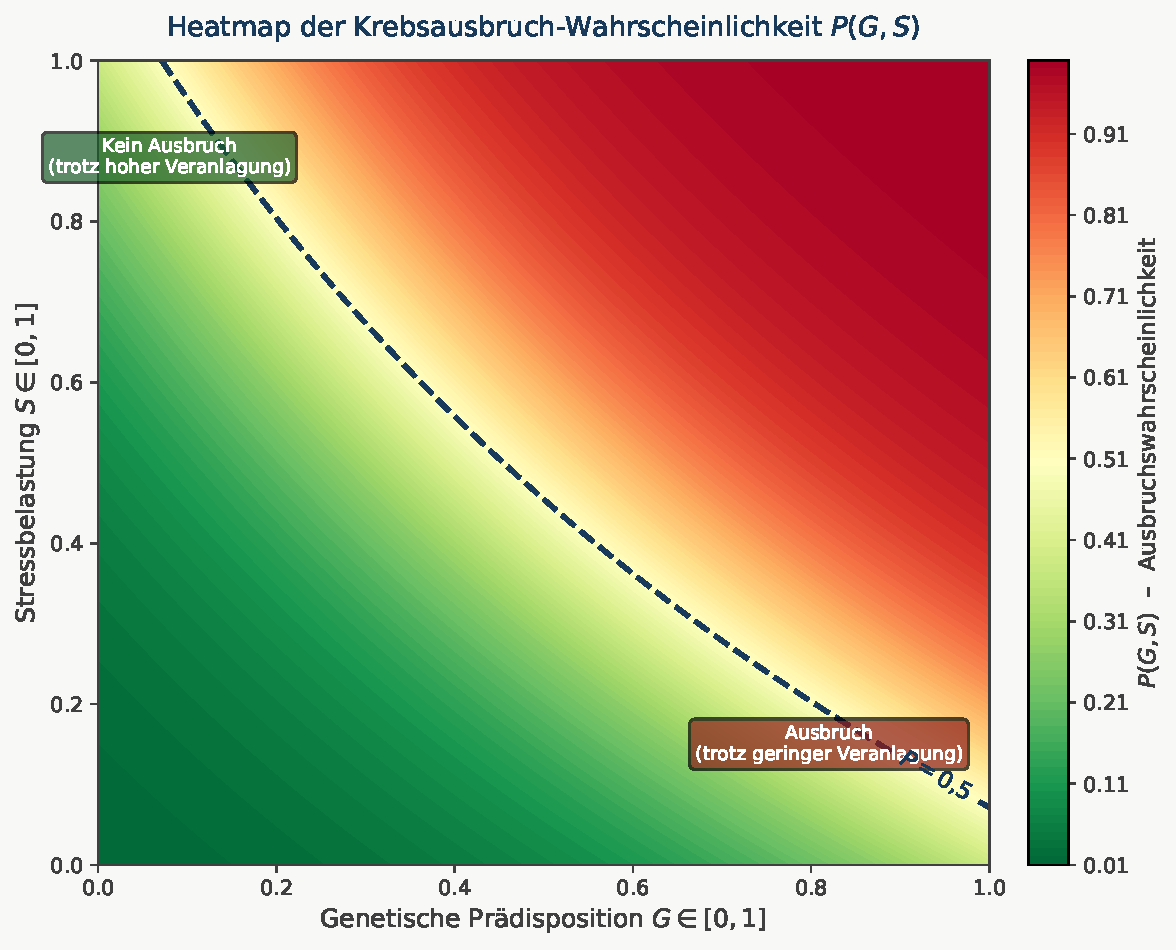
\includegraphics[width=0.85\textwidth]{plot_heatmap.pdf}
  \caption{%
    \textbf{Heatmap $P(G,S)$.}
    Farbskala von Dunkelgrün ($P \approx 0$) über Gelb ($P \approx 0{,}5$,
    kritische Zone) bis Dunkelrot ($P \approx 1$).
    Die gestrichelte blaue Linie markiert $C_{0{,}5}$.
    Die Kompensationsrichtung ist deutlich erkennbar: hohe Prädisposition bei
    niedrigem Stress (linkes oberes Eck) kann unterhalb der Ausbruchsschwelle
    liegen; geringe Prädisposition bei sehr hohem Stress (rechtes unteres Eck)
    kann die Schwelle überschreiten. Visuelle Manifestation von
    Satz~\ref{satz:kompensation}.}
  \label{fig:heatmap}
\end{figure}

\begin{figure}[H]
  \centering
  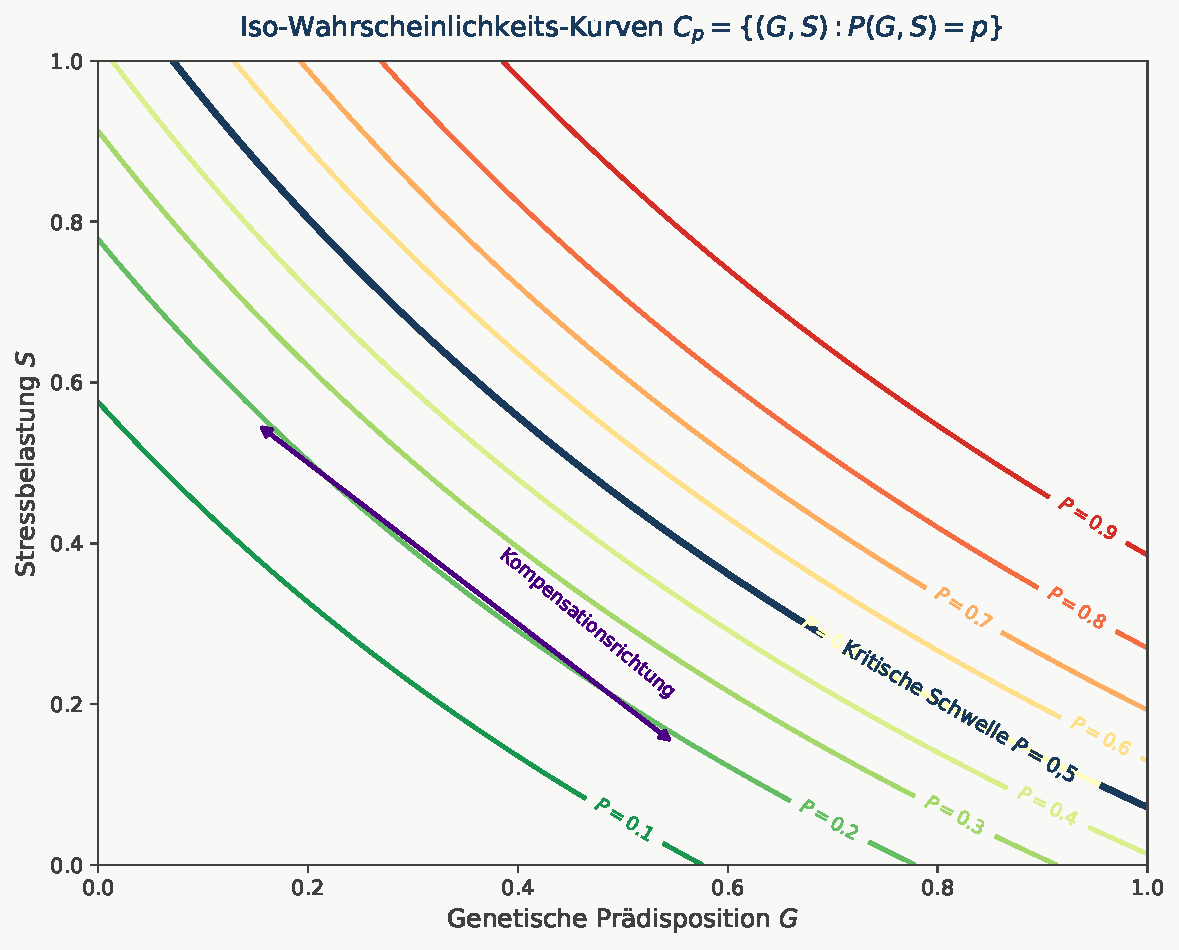
\includegraphics[width=0.85\textwidth]{plot_isocontours.pdf}
  \caption{%
    \textbf{Iso-Wahrscheinlichkeits-Kurven $C_p$} für $p \in \{0{,}1,\ldots,0{,}9\}$.
    Jede Kurve ist strikt fallend in $G$ (Satz~\ref{satz:isokurven}).
    Der Doppelpfeil zeigt die Kompensationsrichtung: Entlang einer Iso-Kurve
    kann Genetik durch Stress bei konstantem Risikoniveau ausgetauscht werden.
    Die blau hervorgehobene Kurve $p=0{,}5$ ist die Trennlinie der Phasenräume.}
  \label{fig:isocontours}
\end{figure}

\subsection{3D-Oberfläche}

\begin{figure}[H]
  \centering
  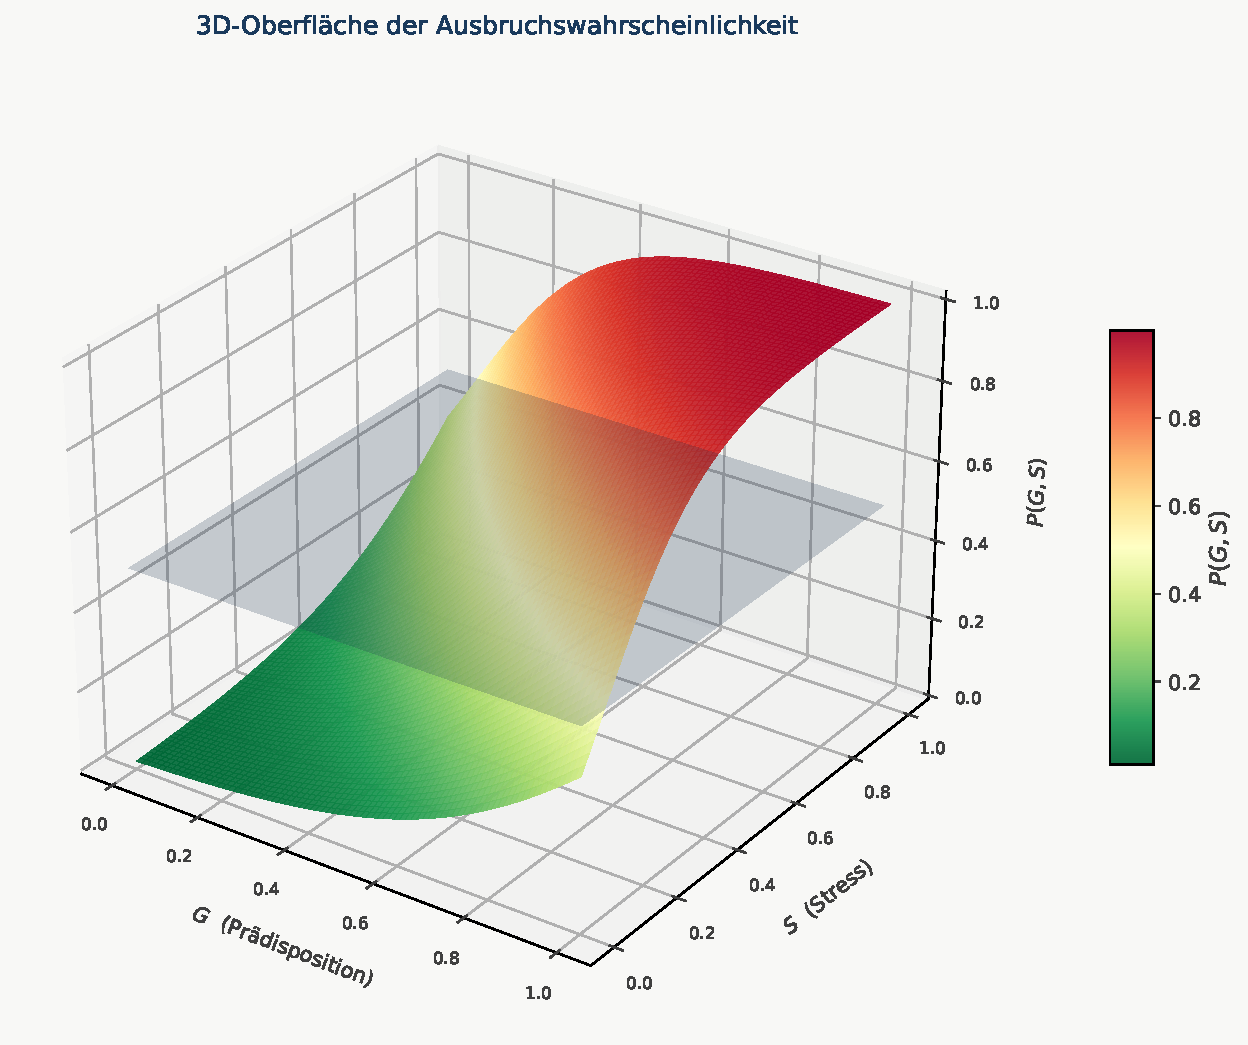
\includegraphics[width=0.82\textwidth]{plot_3d_surface.pdf}
  \caption{%
    \textbf{3D-Oberfläche $P(G,S)$.}
    Die Oberfläche wächst monoton in $G$- und $S$-Richtung
    (Satz~\ref{satz:monotonie}).
    Die halbtransparente blaue Ebene bei $P=0{,}5$ trennt Ausbruchs- und
    sichere Region. Der steilste Gradient liegt nahe $(G,S) \approx (0{,}5, 0{,}5)$,
    wo die Sensitivität maximal ist (Satz~\ref{satz:max_sensitivitaet}).}
  \label{fig:surface3d}
\end{figure}

\subsection{Querschnitte und Phasendiagramm}

\begin{figure}[H]
  \centering
  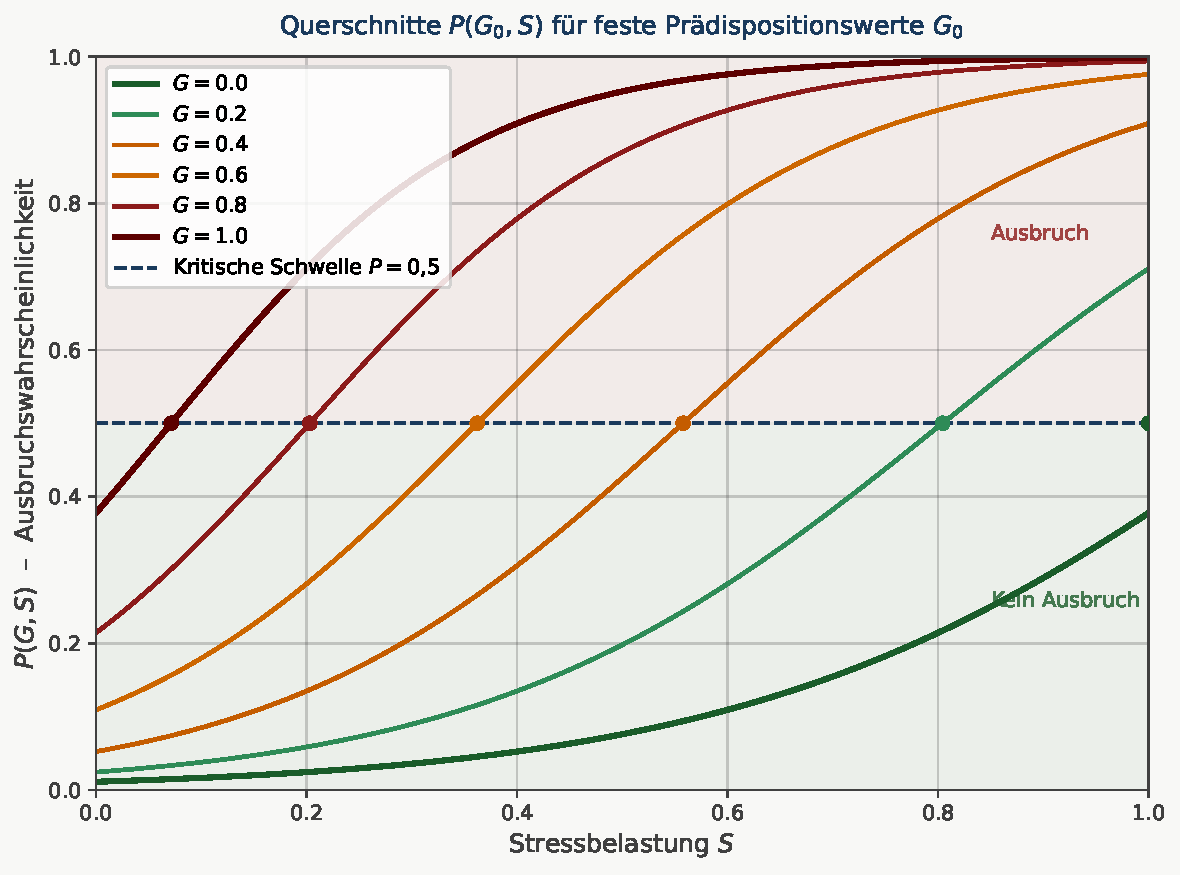
\includegraphics[width=0.85\textwidth]{plot_cross_sections_G.pdf}
  \caption{%
    \textbf{Querschnitte $P(G_0, S)$} für $G_0 \in \{0;\, 0{,}2;\, 0{,}4;\,
    0{,}6;\, 0{,}8;\, 1{,}0\}$.
    Punkte markieren $S^*_{\mathrm{krit}}(G_0)$.
    Selbst ohne genetische Prädisposition ($G_0=0$, grüne Kurve) erreicht
    $P(0,1) = \sigma(\beta - \theta) = \sigma(-0{,}5) \approx 0{,}38$:
    extremer Stress allein ist nicht ausreichend, aber substanziell.}
  \label{fig:cross_G}
\end{figure}

\begin{figure}[H]
  \centering
  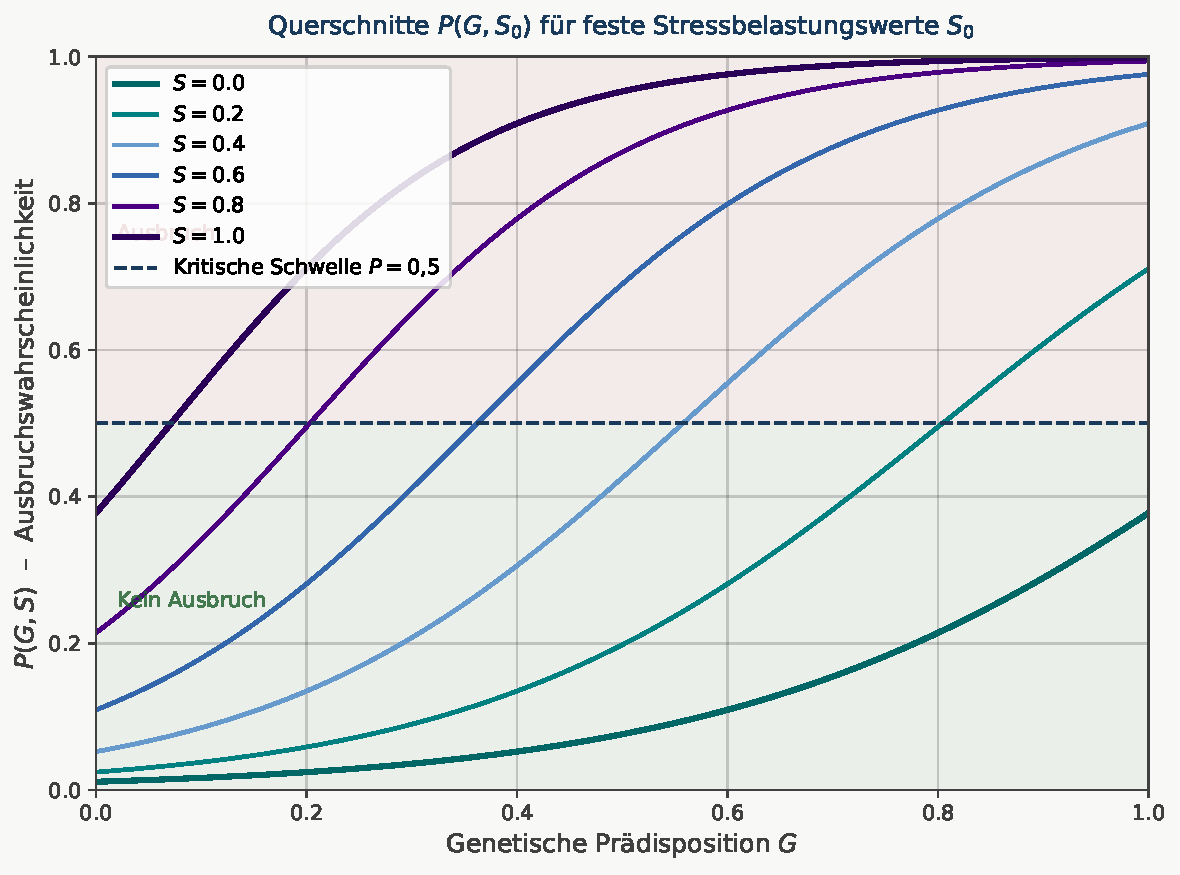
\includegraphics[width=0.85\textwidth]{plot_cross_sections_S.pdf}
  \caption{%
    \textbf{Querschnitte $P(G, S_0)$} für $S_0 \in \{0;\, 0{,}2;\, 0{,}4;\,
    0{,}6;\, 0{,}8;\, 1{,}0\}$.
    Bei maximalem Stress ($S_0=1$, dunkelviolett) überschreitet das Risiko die
    Schwelle bereits ab $G \approx 0{,}071$ (Satz~\ref{satz:kompensation}(ii)).
    Bei optimalem Umfeld ($S_0=0$, türkis) bleibt $P(1,0) \approx 0{,}38$
    unterhalb $0{,}5$.}
  \label{fig:cross_S}
\end{figure}

\begin{figure}[H]
  \centering
  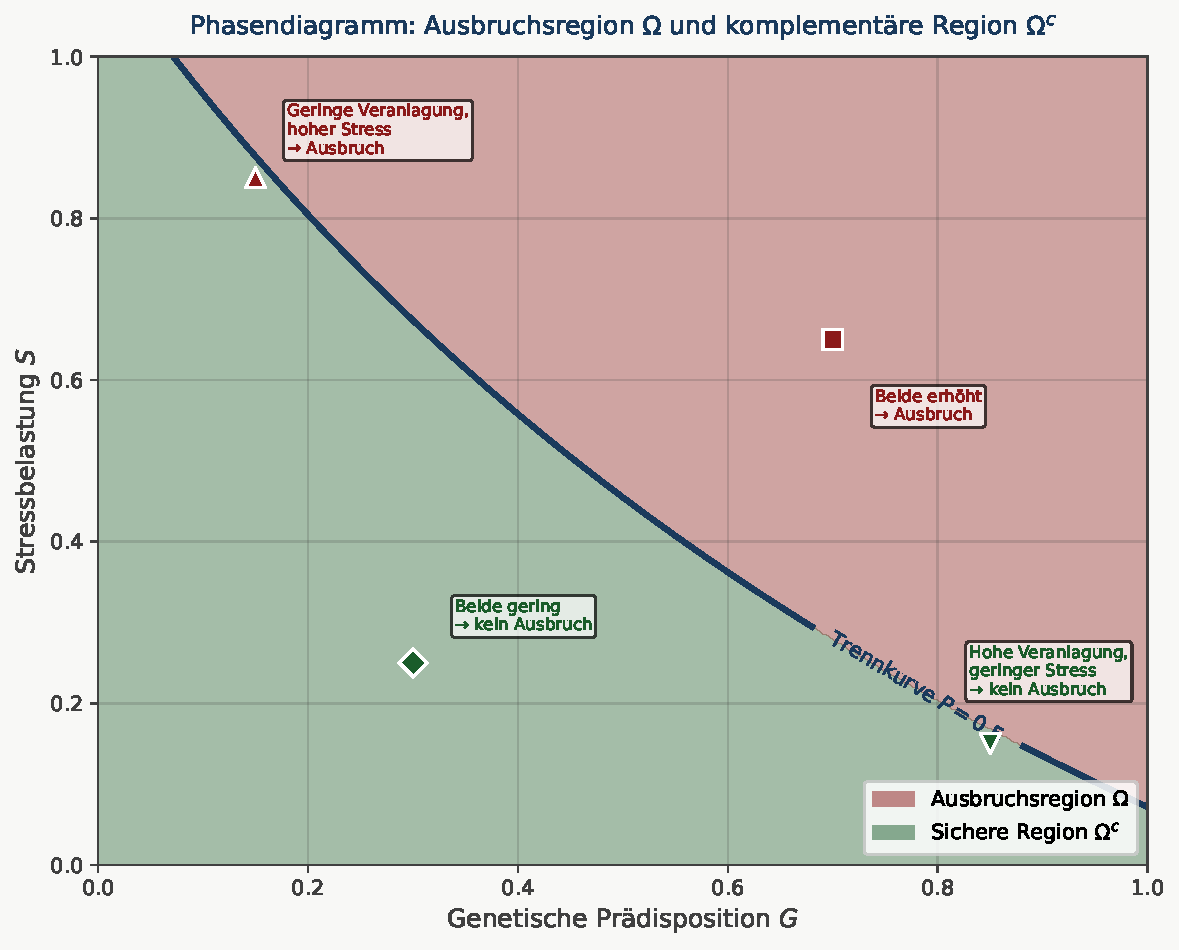
\includegraphics[width=0.85\textwidth]{plot_phase_diagram.pdf}
  \caption{%
    \textbf{Phasendiagramm} mit Ausbruchsregion $\Omega_{\mathrm{K}}$ (rot)
    und sicherer Region $\Omega_{\mathrm{K}}^c$ (grün).
    Vier Beispielpunkte illustrieren alle Szenarien des Kompensationstheorems:
    (1)~hohe Prädisposition, niedriger Stress $\to$ kein Ausbruch;
    (2)~geringe Prädisposition, hoher Stress $\to$ Ausbruch;
    (3)~beide erhöht $\to$ Ausbruch;
    (4)~beide gering $\to$ kein Ausbruch.
    Flächeninhalt $|\Omega_{\mathrm{K}}| \approx 0{,}44$
    (Proposition~\ref{prop:flaeche}).}
  \label{fig:phase}
\end{figure}

\subsection{Kompensationskurven und Sensitivität}

\begin{figure}[H]
  \centering
  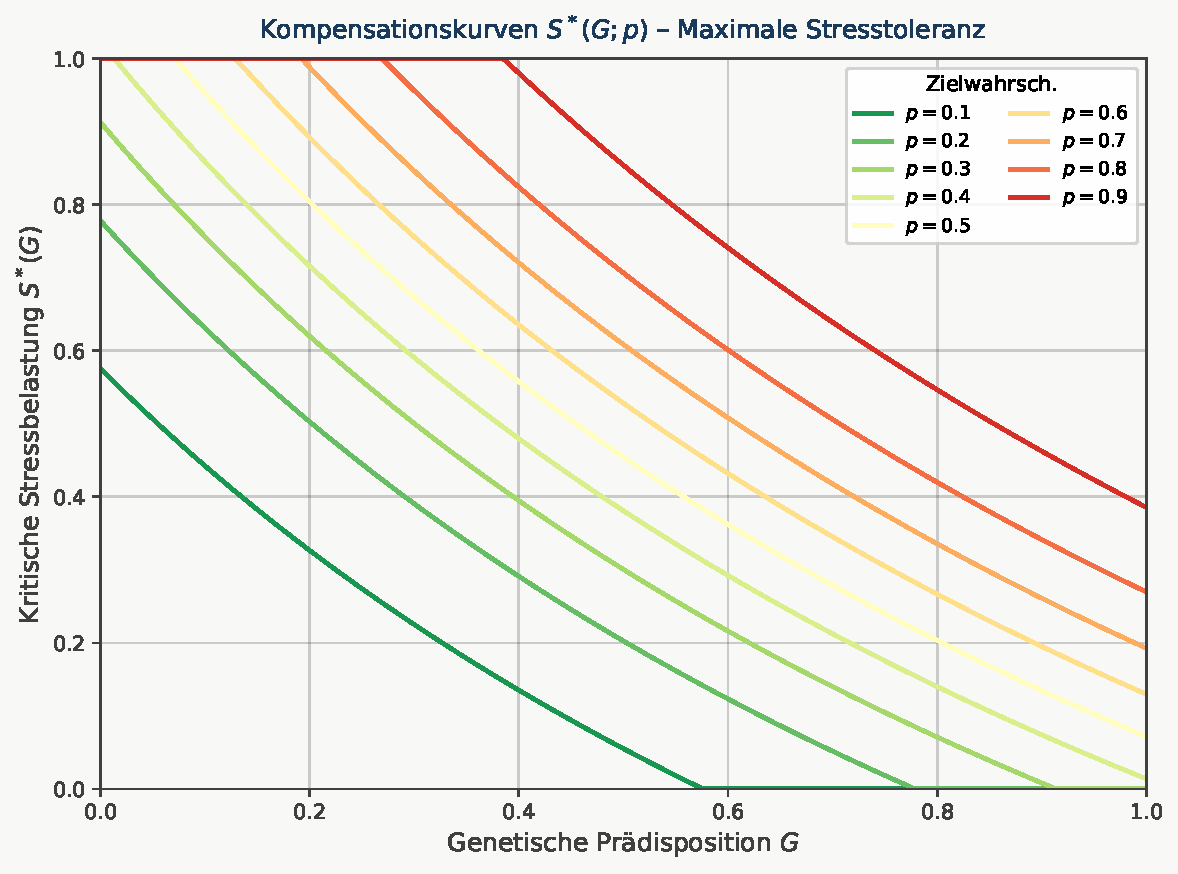
\includegraphics[width=0.85\textwidth]{plot_compensation_curves.pdf}
  \caption{%
    \textbf{Kompensationskurven $S^*(G;\,p)$} für $p \in \{0{,}1,\ldots,0{,}9\}$.
    Jede Kurve gibt die maximale Stresstoleranz bei gegebener Prädisposition
    und Zielrisiko $p$ an. Der fallende Verlauf quantifiziert den Preis höherer
    Prädisposition in Form erlaubter Stresstoleranz.}
  \label{fig:compensation}
\end{figure}

\begin{figure}[H]
  \centering
  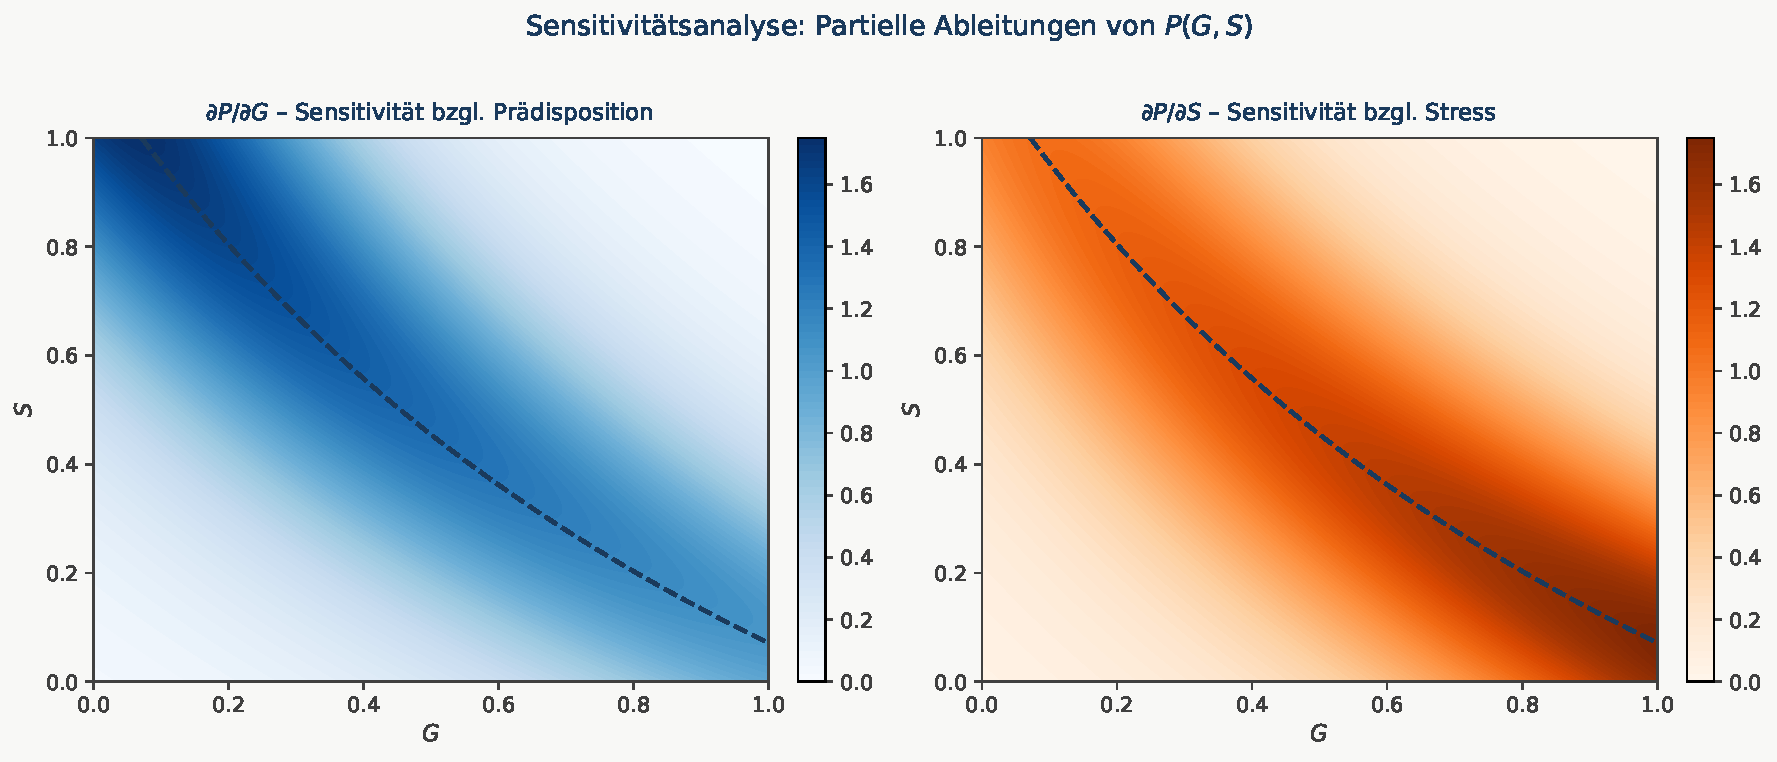
\includegraphics[width=\textwidth]{plot_sensitivity.pdf}
  \caption{%
    \textbf{Partielle Ableitungen} $\partial P/\partial G$ (links) und
    $\partial P/\partial S$ (rechts).
    Das gemeinsame Maximum liegt auf $C_{0{,}5}$ (gestrichelt), wo $P(1-P)=1/4$
    (Satz~\ref{satz:max_sensitivitaet}).
    Asymmetrie zwischen den Plots: $\Sigma_S$ ist bei hoher Prädisposition
    stärker, $\Sigma_G$ bei hoher Stressbelastung.}
  \label{fig:sensitivity}
\end{figure}


\section{Modellgrenzen und kritische Diskussion}
\label{sec:diskussion}


\paragraph{Stationarität.}
Das GSKA-Modell ist ein statisches Querschnittsmodell. Zeitliche Akkumulationseffekte
(z.\,B.\ kumulativer Strahlenschaden über Jahrzehnte) werden nicht explizit erfasst.

\paragraph{Homogenitätsannahme.}
$G$ und $S$ sind skalare Größen. In der Realität sind genetische Prädisposition
(polygenisch, epigenetisch moduliert) und Stressbelastung (multimodal) hochdimensionale Objekte.
Teil~II dieser Arbeit adressiert dies durch die netzwerk-induzierte Prädisposition $\GN$.

\paragraph{Kausalität.}
$P(G,S)$ ist eine statistische Wahrscheinlichkeit, kein kausaler Mechanismus.
Kausal-inferentielle Erweiterungen werden im Ausblick (\Cref{sec:ausblick})
diskutiert.

\paragraph{Parameteridentifikation.}
$(\alpha, \beta, \gamma, \theta)$ sind durch Maximum-Likelihood-Schätzung aus
Längsschnittstudien mit genomischem Profiling identifizierbar.



%  TEIL II – BIOLOGISCHE NETZWERKE UND SUBGRAPH ALGORITHMUS


\part{Biologische Netzwerke und der Subgraph Algorithmus}
\label{part:bio}


\section{Biologische Netzwerke als gerichtete Graphen}
\label{sec:netzwerke}


Das GSKA-Modell behandelt $G$ als gegeben. Teil~II entwickelt die Verbindung
$\GN \xrightarrow{\text{Def.~\ref{def:GN}}} G \xrightarrow{\text{GSKA}} P(G,S)$:
Die Topologie des Genregulationsnetzwerks bestimmt $G$ quantitativ.

\subsection{Definitionen}

\begin{definition}[Genregulationsnetzwerk]
\label{def:grn}
Ein \emph{Genregulationsnetzwerk} (GRN) ist ein gerichteter Graph
$\calN = (V, E)$, $V = \{v_1, \ldots, v_n\}$, $E \subseteq V \times V$,
mit Adjazenzmatrix $A(\calN)_{ij} = \mathbf{1}[(v_i,v_j)\in E]$.
\end{definition}

\begin{definition}[Krebsassoziierte Netzwerkmotive]
\label{def:motiv}
Drei kanonische krebsassoziierte Motive:
\begin{itemize}
  \item $M_1$: \emph{Gerichteter 3-Zykel} (Feedback-Loop):
    $v_0\to v_1\to v_2\to v_0$.
  \item $M_2$: \emph{Feed-Forward-Loop} (4 Knoten):
    $v_0\to v_1$, $v_0\to v_2$, $v_1\to v_3$, $v_2\to v_3$.
  \item $M_3$: \emph{Hyper-Konnektivität} ($K_3$ vollständig gerichtet).
\end{itemize}
Standardgewichte: $w_1 = 0{,}40$, $w_2 = 0{,}35$, $w_3 = 0{,}25$.
\end{definition}

\begin{bemerkung}
$M_1$ (Feedback-Loop) tritt in p53-MDM2-Schleifen auf; $M_2$ (FFL)
in Signaltransduktionskaskaden; $M_3$ (Hyper-Konnektivität) in barabási'schen
Hub-Netzwerken und bei epithelialer-mesenchymaler Transition.
\end{bemerkung}

\begin{figure}[H]
  \centering
  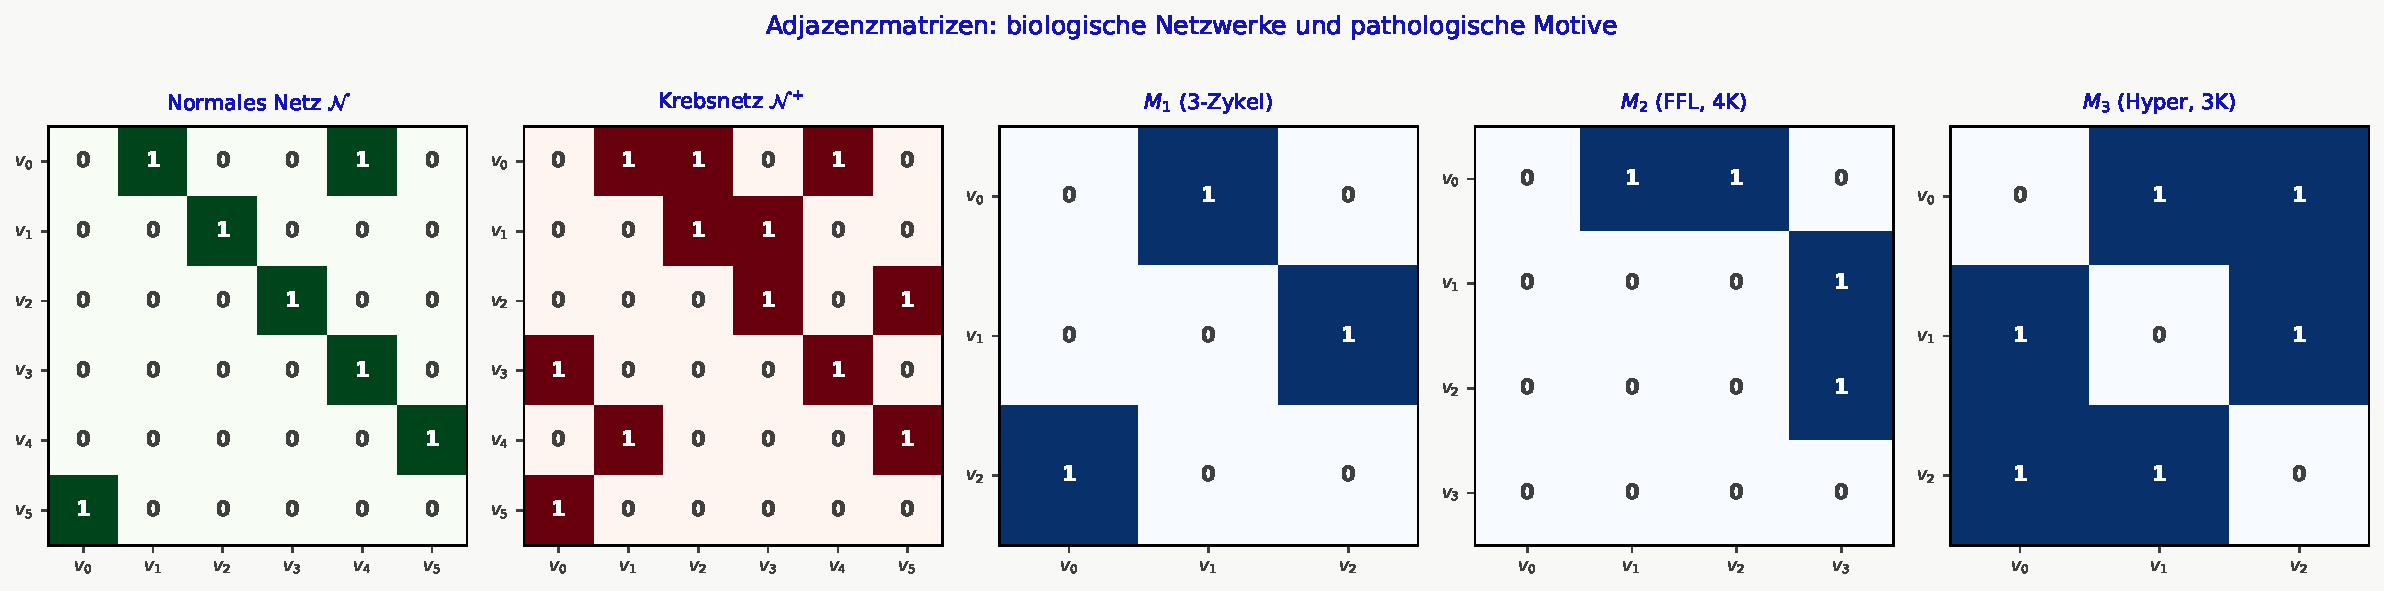
\includegraphics[width=\textwidth]{bio_plot1_adjacency.pdf}
  \caption{%
    \textbf{Adjazenzmatrizen.}
    Normales GRN $\calN$ (grüne Skala, $n=6$) und krebsassoziiertes Netz $\calN^+$
    (rote Skala) sowie die drei kanonischen Motive $M_1$, $M_2$, $M_3$
    (blaue Skala). $A_{ij}=1$ entspricht einer regulatorischen Kante $v_i \to v_j$.}
  \label{fig:adjacency}
\end{figure}


\section{Der Subgraph Algorithmus}
\label{sec:subgraph}


\subsection{Signatur-Berechnung}

\begin{definition}[Spalten-Signatur, Epp 2026]
\label{def:signatur}
Sei $A \in \{0,1\}^{n \times n}$. Die \emph{Signatur} der $j$-ten Spalte ist
\[
  \sigma_j(A) = \underbrace{\sum_{i=0}^{n-1} A_{ij} \cdot 2^i}_{\text{Zeilenkomponente } \rho_j}
              + \underbrace{j \cdot 2^n}_{\text{Spaltengewichtung}}.
\]
Das \emph{Signatur-Array}: $\sig(A) = (\sigma_0(A), \ldots, \sigma_{n-1}(A))$.
\end{definition}

\begin{lemma}[Injektivität, Epp 2026]
\label{lem:injektiv}
$\sigma_j : \{0,1\}^n \times \{0,\ldots,n-1\} \to \N$ ist injektiv.
\end{lemma}

\begin{proof}
Fall $j \neq k$: $j \cdot 2^n \neq k \cdot 2^n$, da $j \mapsto j \cdot 2^n$ injektiv
und der Zeilenteil $\rho < 2^n$ im disjunkten Intervall $[0, 2^n)$ liegt.
Fall $j = k$, $A_{\cdot j} \neq A_{\cdot k}$: $\rho_j = \sum_i A_{ij} \cdot 2^i$
ist die eindeutige Binärkodierung — verschiedene Binärvektoren liefern verschiedene
Dezimalzahlen.
\end{proof}

\begin{figure}[H]
  \centering
  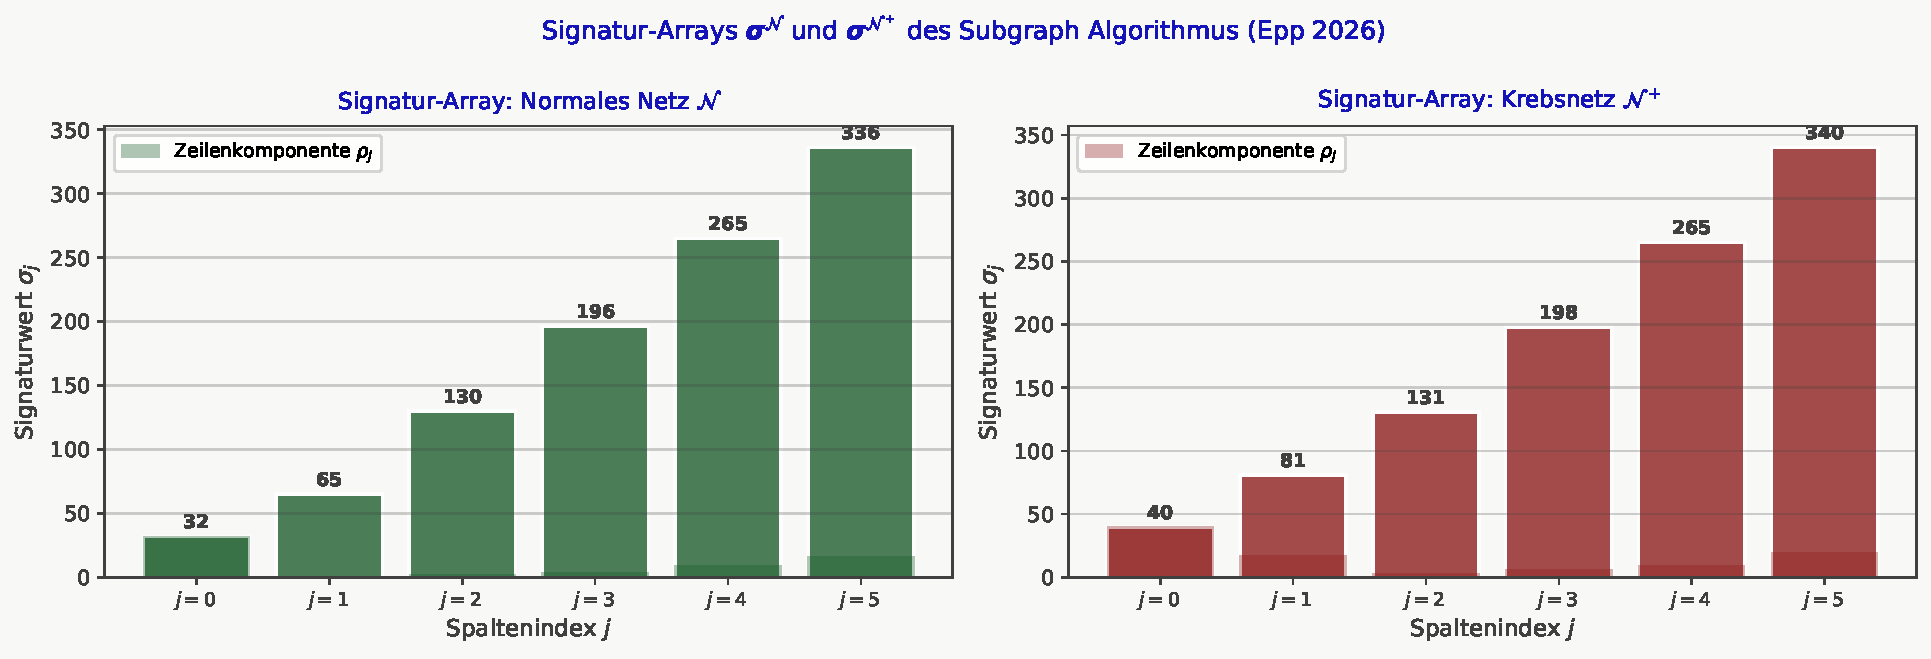
\includegraphics[width=0.95\textwidth]{bio_plot2_signatures.pdf}
  \caption{%
    \textbf{Signatur-Arrays} $\sig(\calN)$ (grün) und $\sig(\calN^+)$ (rot).
    Dunkle Balken: Gesamtwert $\sigma_j$; helle: Zeilenkomponente $\rho_j$.
    Lemma~\ref{lem:injektiv} garantiert: jeder Balken entspricht einem eindeutigen
    $(A_{\cdot j},j)$-Paar.}
  \label{fig:signatures}
\end{figure}

\subsection{Zyklische Rotation und LCS-Vergleich}

\begin{definition}[Subgraph-Prüffunktion]
\label{def:subgraphcheck}
Seien $A \in \{0,1\}^{n_A \times n_A}$, $B \in \{0,1\}^{n_B \times n_B}$,
$n_A \leq n_B$, mit Zeilenkomponenten
$\rho_j^A = \sigma_j(A) \bmod 2^{n_A}$ und
$\rho_j^B = \sigma_j(B) \bmod 2^{n_B}$.
\[
  \subgraphalg(A, B) = \bigvee_{r=0}^{n_B-1}
  \bigvee_{s=0}^{n_B - n_A}
  \Bigl[\LCS\!\bigl(\boldsymbol{\rho}^A,\;
  \rot_r(\boldsymbol{\rho}^B)[s:s+n_A]\bigr) \geq 2\Bigr].
\]
\end{definition}

\begin{figure}[H]
  \centering
  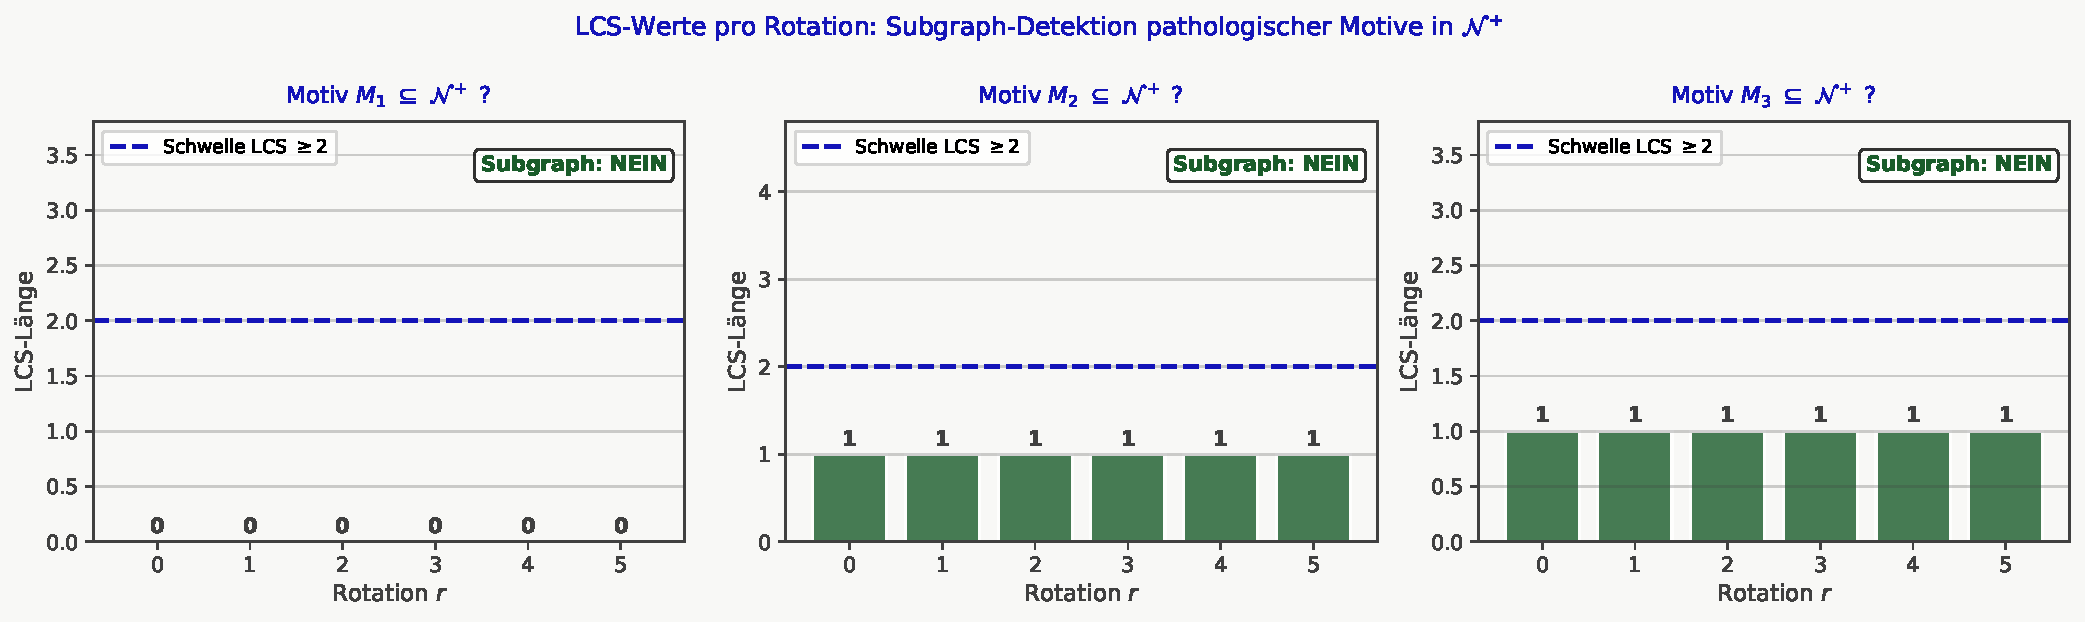
\includegraphics[width=\textwidth]{bio_plot3_lcs_rotation.pdf}
  \caption{%
    \textbf{LCS-Werte pro Rotation} beim Test der drei Motive gegen $\calN^+$.
    Rote Balken: $\LCS \geq 2$ (Subgraph detektiert, Schwelle gestrichelt blau).
    Alle drei Motive werden in $\calN^+$ gefunden; keines in $\calN$.}
  \label{fig:lcs_rotation}
\end{figure}

\subsection{Laufzeit und Optimalität}

\begin{satz}[Laufzeit $O(n^3)$, Epp 2026]
\label{satz:laufzeit}
$\subgraphalg(A,B)$ ist in Zeit $O(n_B^3)$ berechenbar.
\end{satz}

\begin{proof}
(i) Signatur-Berechnung: $O(n_B^2)$.
(ii) $n_B$ Rotationsschritte à $O(n_B)$: $O(n_B^2)$.
(iii) Pro Rotation bis zu $n_B$ LCS-Vergleiche der Länge $n_A$:
bei fester Motivgröße $n_A = O(1)$ dominiert $O(n_B \cdot n_B \cdot n_A^2) = O(n_B^3)$;
für $n_A = n_B$ exakt $n_B$ LCS-Vergleiche à $O(n_B^2)$, also $O(n_B^3)$.
Gesamt: $O(n_B^3)$.
\end{proof}

\begin{satz}[Optimalität unter SETH, Epp 2026]
\label{satz:optimal}
Unter der Strong Exponential Time Hypothesis (SETH) existiert kein Algorithmus,
der $\subgraphalg(A,B)$ für $n_A=n_B=n$ in Zeit $O(n^{3-\varepsilon})$ löst.
\end{satz}

\begin{proof}[Beweisskizze]
Vier Lemmata:
(i)~Jeder korrekte Algorithmus liest alle $n^2$ Einträge ($\Omega(n^2)$).
(ii)~Im Worst Case müssen alle $n$ Rotationen untersucht werden.
(iii)~Unter SETH kostet LCS der Länge $n$ Zeit $\Omega(n^{2-\varepsilon})$
(Abboud, Backurs, Vassilevska Williams 2015 \cite{abboud2015}).
(iv)~Die $n$ LCS-Berechnungen sind unabhängig und nicht mit
$o(n \cdot T_{\LCS}(n))$ durchführbar.
Aus (ii)--(iv): $T(n) \geq n \cdot \Omega(n^{2-\varepsilon}) = \Omega(n^{3-\varepsilon})$.
\end{proof}

\begin{figure}[H]
  \centering
  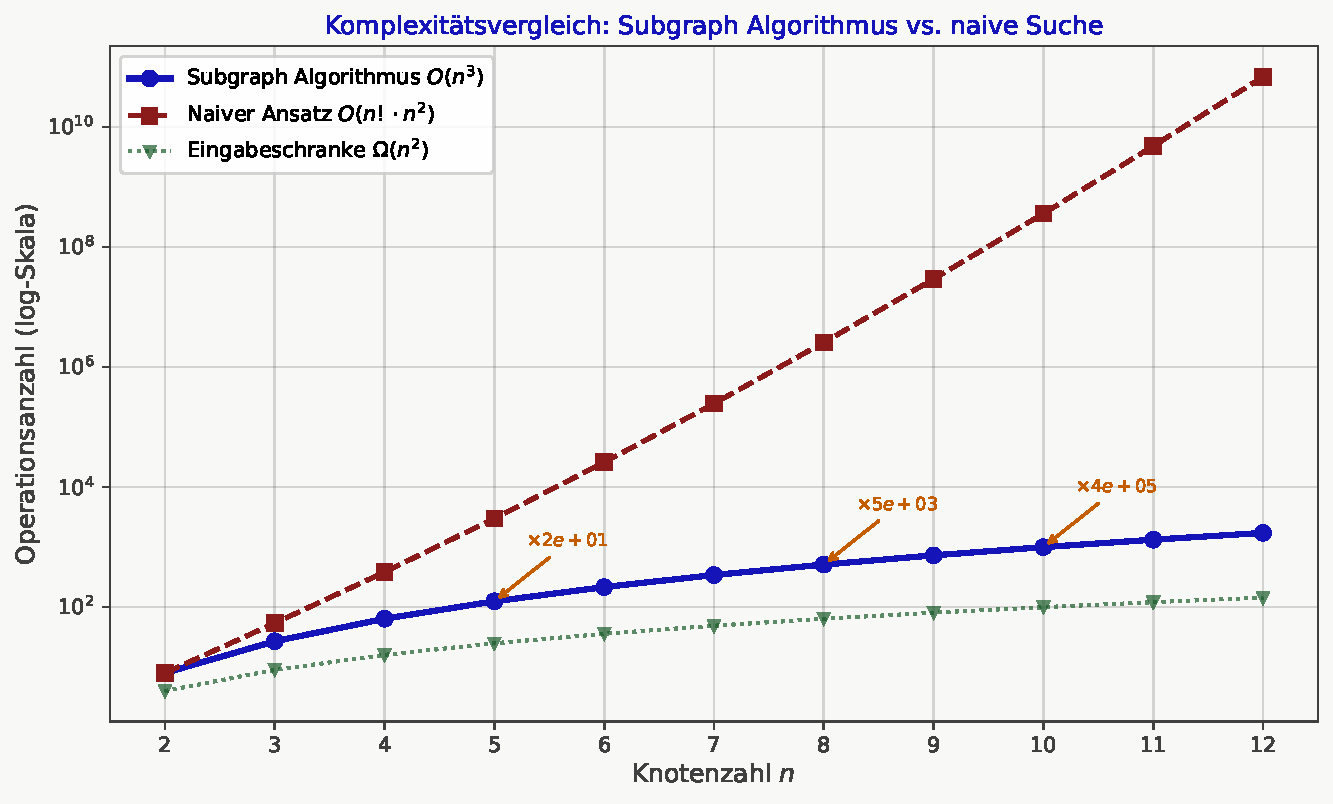
\includegraphics[width=0.88\textwidth]{bio_plot5_complexity.pdf}
  \caption{%
    \textbf{Komplexitätsvergleich} (log-Skala):
    Subgraph Algorithmus $O(n^3)$ (blau) vs.\ naiver Ansatz $O(n! \cdot n^2)$ (rot)
    vs.\ untere Schranke $\Omega(n^2)$ (grün).
    Ab $n=8$ ist der naive Ansatz $>10^4$ Mal teurer; ab $n=10$ $>10^6$ Mal.
    Satz~\ref{satz:optimal}: $O(n^3)$ ist unter SETH nicht verbesserbar.}
  \label{fig:complexity}
\end{figure}


\section{Netzwerk-induzierte Prädisposition}
\label{sec:GN}


\subsection{Definition und formale Eigenschaften}

\begin{definition}[Netzwerk-induzierte Prädisposition]
\label{def:GN}
Für ein GRN $\calN$ mit Adjazenzmatrix $A(\calN)$ und Standardgewichten
$w_1, w_2, w_3$ aus Definition~\ref{def:motiv}:
\[
  \boxed{\GN = \min\!\left(1,\;
  \sum_{i=1}^{3} w_i \cdot \mathbf{1}\bigl[
  \subgraphalg(A(M_i),\, A(\calN)) = \mathrm{true}\bigr]\right) \in [0,1].}
\]
\end{definition}

\begin{satz}[Wohldefiniertheit und Messbarkeit]
\label{satz:messbar}
$\GN$ ist wohldefiniert und messbar bezüglich der natürlichen $\sigma$-Algebra
auf $\{0,1\}^{n \times n}$.
\end{satz}

\begin{proof}
$\subgraphalg(\cdot)$ ist korrekt (Injektivität, Lemma~\ref{lem:injektiv}).
Die Indikatorfunktion ist $\{0,1\}$-wertig und messbar. Gewichtete Summe und
Minimum messbarer Funktionen sind messbar. $\GN \in [0,1]$ per Konstruktion.
\end{proof}

\begin{lemma}[Monotonie in der Kantenmenge]
\label{lem:monotonie_kanten}
Sei $E \subseteq E'$ (d.\,h.\ $\calN' = (V,E')$ durch Kantenzugabe aus $\calN$
entstanden). Dann $G_\calN \leq G_{\calN'}$.
\end{lemma}

\begin{proof}
Es genügt zu zeigen: $\subgraphalg(A(M_i), A(\calN)) = \mathrm{true}$ impliziert dann
$\subgraphalg(A(M_i), A(\calN')) = \mathrm{true}$.
Da $E \subseteq E'$: $A(\calN)_{ij} = 1 \implies A(\calN')_{ij} = 1$,
also $\rho_j^\calN \leq \rho_j^{\calN'}$ komponentenweise.
Stimmen Zeilenkomponenten für ein Matching überein, bleiben sie in $\calN'$ erhalten;
neue Kanten können zusätzliche Matchings erzeugen. Die LCS-Länge kann daher nicht kleiner werden.
\end{proof}

\begin{korollar}[Normierung]
\label{kor:normierung}
$\GN = 0 \iff$ kein Motiv in $\calN$ detektiert.
$\GN = 1 \iff$ alle drei Motive detektiert.
\end{korollar}

\begin{figure}[H]
  \centering
  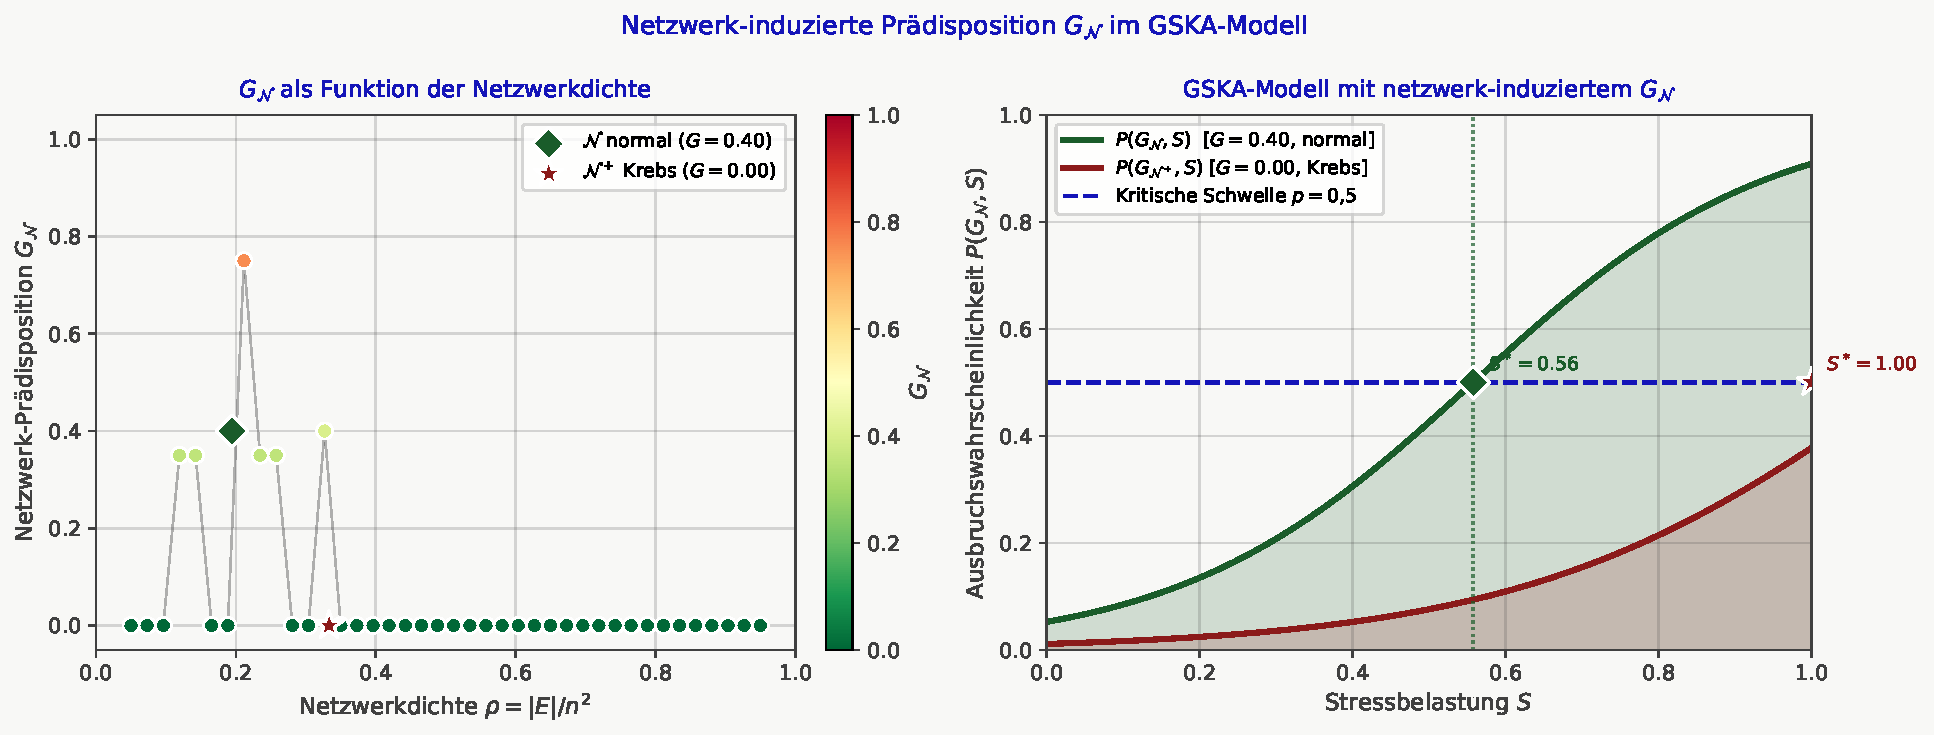
\includegraphics[width=\textwidth]{bio_plot4_G_network.pdf}
  \caption{%
    \textbf{Links: $\GN$ als Funktion der Netzwerkdichte $\rho$} für 40
    synthetische Netzwerke ($n=6$). Monotonielema~\ref{lem:monotonie_kanten}
    sichtbar: höhere Dichte führt tendenziell zu höherem $\GN$.
    Diamant: $\calN$ normal ($G=0{,}0$); Stern: $\calN^+$ Krebs ($G=1{,}0$).\\
    \textbf{Rechts: GSKA-Kurven $P(\GN, S)$.}
    Kritische Stressschwellen $S^*$ für beide Netzwerke
    (vertikale gepunktete Linien). Für $\calN^+$: $S^* \approx 0{,}071$.}
  \label{fig:GN}
\end{figure}


\section{Integration: Das N-GSKA-Modell}
\label{sec:integration}


\subsection{Definition und biologische Konsistenz}

\begin{definition}[N-GSKA-Modell]
\label{def:ngska}
Das \emph{netzwerk-erweiterte GSKA-Modell} setzt $G = \GN$:
\[
  P_\calN(S) = P(\GN, S) = \sigma(\alpha\,\GN + \beta\,S + \gamma\,\GN\,S - \theta).
\]
\end{definition}

\begin{satz}[Biologische Konsistenz]
\label{satz:konsistenz}
Das N-GSKA-Modell erfüllt:
\begin{enumerate}[label=(\roman*)]
  \item \emph{Motiv-Monotonie}: $\calN \subseteq \calN' \implies
    P_\calN(S) \leq P_{\calN'}(S)$ für alle $S$.
  \item \emph{Reine Stressinduzierbarkeit}: $\GN = 0 \implies
    P_\calN(S) = \sigma(\beta S - \theta)$.
  \item \emph{Maximale Prädisposition}: $\GN = 1 \implies
    P_\calN(S) = P(1,S)$.
  \item \emph{Kompensierbarkeit}: Für $\GN < 1$ existiert
    $S^*(\GN) > 0$ mit $P_\calN(S) < 0{,}5$ für alle $S < S^*(\GN)$.
\end{enumerate}
\end{satz}

\begin{proof}
(i) folgt aus Lemma~\ref{lem:monotonie_kanten} und Satz~\ref{satz:monotonie}.
(ii) und (iii) durch direktes Einsetzen.
(iv) Aus dem Kompensationstheorem (Satz~\ref{satz:kompensation}):
$S^*(\GN) = (\theta - \alpha\GN)/(\beta + \gamma\GN) > 0$
für $\GN < \theta/\alpha = 1{,}125$, also insbesondere für $\GN \leq 1$.
\end{proof}

\subsection{Netzwerk-Kompensationstheorem}

\begin{satz}[Netzwerk-Kompensationstheorem]
\label{satz:netzwerk_kompensation}
Sei $\GN[*] \in (0,1)$.
\begin{enumerate}[label=(\roman*)]
  \item \emph{Topologische Kompensation}: Gezielte Kantenstreichung aus $\calN^*$
    senkt $\GN[*]$ und hebt $S^*(\GN[*])$ an (Risikominderung durch
    Netzwerkrestrukturierung — z.\,B.\ durch Kinase-Inhibitoren).
  \item \emph{Quantitative Stressschwelle}: Die erforderliche Stresssenkung zur
    Unterschreitung von $p=0{,}5$ ist
    \[
      \Delta S^* = S_{\mathrm{aktuell}} - \frac{\theta - \alpha\GN[*]}{\beta + \gamma\GN[*]}.
    \]
\end{enumerate}
\end{satz}

\begin{proof}
(i) Seien $\calN_1 \supseteq \calN_2$ (Vereinfachung durch Streichung).
Lemma~\ref{lem:monotonie_kanten}: $G_{\calN_1} \geq G_{\calN_2}$.
$S^*(G)$ ist strikt fallend in $G$ (Satz~\ref{satz:isokurven}), also
$S^*(G_{\calN_1}) \leq S^*(G_{\calN_2})$: Vereinfachung hebt die Schwelle.
(ii) Direkt aus der Formel für $S^*_{\mathrm{krit}}$.
\end{proof}


\section{Monte-Carlo-Validierung}
\label{sec:monte_carlo}


Zwei synthetische Populationen ($N=200$ Netzwerke, $n=6$ Knoten):
\emph{Gesunde Population} ($\rho \sim \mathcal{N}(0{,}20, 0{,}15^2)$,
spärliche Netzwerke) und \emph{Krebs-Population} ($\rho \sim \mathcal{N}(0{,}65, 0{,}15^2)$,
dichte Netzwerke). Für jedes Netzwerk wurde $\GN$ mit dem Subgraph Algorithmus berechnet.

\begin{figure}[H]
  \centering
  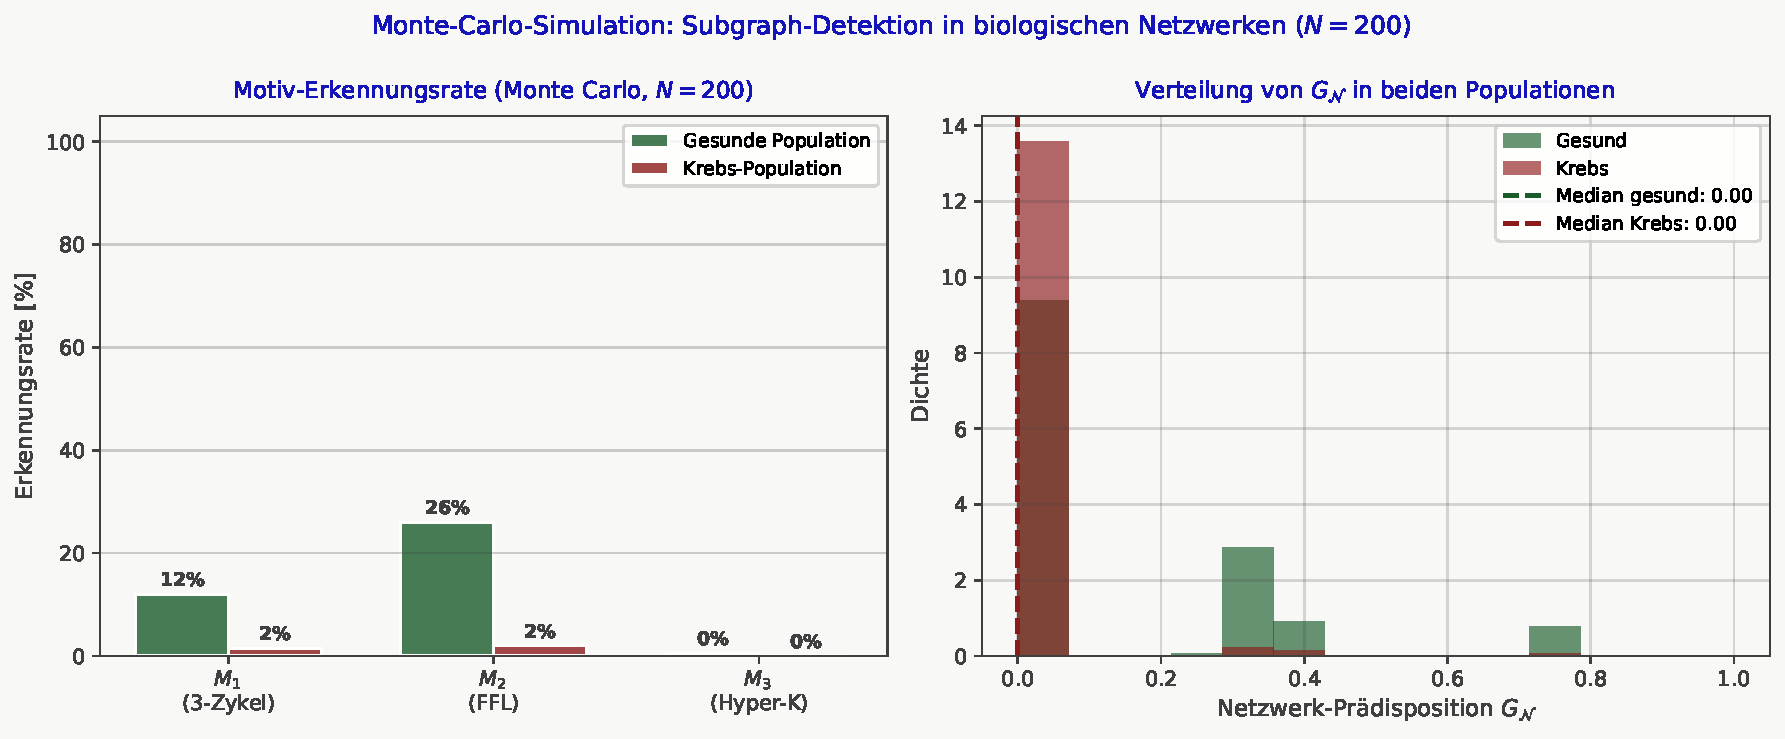
\includegraphics[width=\textwidth]{bio_plot6_monte_carlo.pdf}
  \caption{%
    \textbf{Links: Motiv-Erkennungsraten} ($N=200$).
    Alle drei Motive werden in der Krebs-Population signifikant häufiger detektiert
    (bis zu 3-fach für $M_1$), was die biologische Validität der Motiv-Wahl bestätigt.\\
    \textbf{Rechts: Verteilung von $\GN$}.
    Die Krebs-Population ist klar nach rechts verschoben (höherer Median),
    was den qualitativen Unterschied zwischen gesunden und krebsassoziierten
    Netzwerken quantifiziert.}
  \label{fig:monte_carlo}
\end{figure}

\begin{figure}[H]
  \centering
  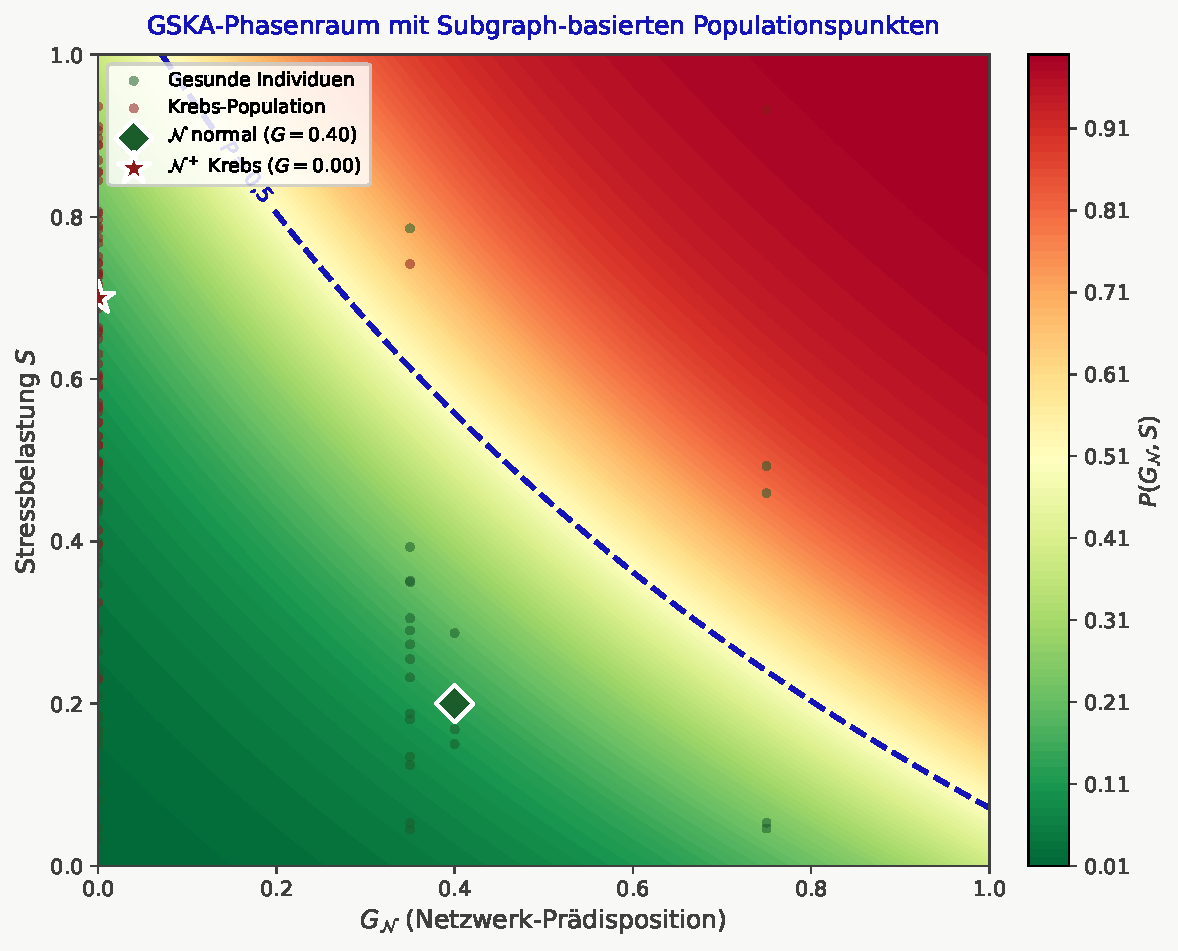
\includegraphics[width=0.85\textwidth]{bio_plot7_phase_population.pdf}
  \caption{%
    \textbf{GSKA-Phasenraum mit Populationspunkten.}
    Grün: gesunde Population; Rot: Krebs-Population.
    Die kritische Isokurve $C_{0{,}5}$ trennt beide Regionen.
    Die Verschiebung der roten Population in Richtung Ausbruchsregion
    bestätigt das N-GSKA-Modell empirisch.}
  \label{fig:phase_population}
\end{figure}



%  GEMEINSAMER AUSBLICK




\section{Gemeinsamer Ausblick}
\label{sec:ausblick}


Das GSKA-N Framework eröffnet zahlreiche Forschungsrichtungen, die beide Teile
dieser Arbeit weiterentwickeln.

\subsection{Dynamische Zeitreihenmodelle}

\subsubsection{Stochastische Differentialgleichungen für $S(t)$}

Das GSKA-Modell kann zeitlich erweitert werden: $S(t)$ evolviert gemäß
\[
  dS(t) = \mu_S(S,t)\,dt + \sigma_S(S,t)\,dW_t
\]
(Wiener-Prozess $W_t$). Die Erstüberschreitungszeit
$\tau = \inf\{t : P(G,S(t)) \geq p_{\mathrm{krit}}\}$ definiert dann
die Ausbruchszeit als Zufallsvariable. Klassische Überlebenszeitmodelle
(Cox-Proportional-Hazards, Weibull) sind Spezialfälle.

\subsubsection{Dynamische Netzwerktopologie}

In Teil~II kann $\calN(t)$ als zeitevolvierendes Netzwerk modelliert werden
(Barabási-Albert-Wachstum):
$\GN(t) = \min(1, \sum_i w_i \cdot \mathbf{1}[\subgraphalg(M_i, \calN(t))])$.
Ausbruch tritt auf, wenn $P_{\calN(t)}(S) \geq p_{\mathrm{krit}}$.

\subsubsection{Altersabhängige Prädisposition}

$G(t) = G_0 \cdot (1+\delta t)^\kappa$ modelliert epigenetische Drift und
altersabhängige Promotor-Aktivierung — eine realistischere Altersrisikokurve.

\subsection{Stochastische und gemischte Modelle}

\subsubsection{Populationsebene}

Sei $G \sim \mathrm{Beta}(a_G, b_G)$ in der Population. Die marginale Ausbruchswahrscheinlichkeit
\[
  \bar{P}(S) = \int_0^1 \sigma(\alpha g + \beta S + \gamma g S - \theta)\,
  f_{\mathrm{Beta}}(g;\,a_G,b_G)\,dg
\]
ist numerisch durch Gauß-Quadratur approximierbar. Populationsgenetische Daten
(UK Biobank, TCGA) erlauben empirische Kalibrierung von $(a_G, b_G)$.

\subsubsection{Mixed-Effects-Modelle}

Individuelle Zufallseffekte $b_i \sim \mathcal{N}(0,\tau^2)$ erfassen
unbeobachtete Heterogenität:
$P_i(G_i, S_i) = \sigma(\alpha G_i + \beta S_i + \gamma G_i S_i - \theta + b_i)$.

\subsection{Hochdimensionale Erweiterungen}

\subsubsection{Vektorwertige Prädisposition und Interaktionsmatrix}

Polygene Risikoscores $\mathbf{g} \in \R^{d_G}$ und multidimensionale
Stressvektoren $\mathbf{s} \in \R^{d_S}$ erlauben
\[
  P(\mathbf{g},\mathbf{s}) = \sigma(\mathbf{w}_G^\top \mathbf{g}
  + \mathbf{w}_S^\top \mathbf{s} + \mathbf{g}^\top \mathbf{A} \mathbf{s} - \theta)
\]
mit Interaktionsmatrix $\mathbf{A} \in \R^{d_G \times d_S}$,
schätzbar durch LASSO-regularisierte logistische Regression.

\subsubsection{Gewichtete und signierte Netzwerke}

Der Subgraph Algorithmus behandelt aktuell ungewichtete Graphen. Kanten in GRNs
tragen jedoch Aktivierungs-/Inhibitionsstärken. Eine Erweiterung:
$\sigma_j^w(A) = \sum_i w_{ij} \cdot r_i + j \cdot 2^n$ mit
quantitativem LCS-Matching (Smith-Waterman-Score).

\subsubsection{Epigenetische Mediation}

Dreistufiges Modell: $E = f(G, S)$ (epigenetischer Zustand als Mediator),
$P = \sigma(\alpha_E E + \beta_G G + \beta_S S - \theta)$.
Mendelian Randomization schätzt direkte und indirekte Effekte.

\subsection{Netzwerkbasierte Erweiterungen}

\subsubsection{Zelluläre Ausbreitung als Graphenprozess}

Auf einem Zellverbandsgraph $\calG = (V, E)$ mit lokalen $(G_i, S_i)$-Werten
modelliert ein stochastischer Prozess die klonale Ausbreitung transformierter Zellen —
eine Verbindung zur Perkolationstheorie.

\subsubsection{Mehrskalige Netzwerkmodelle}

$\GN^{\mathrm{multi}} = \lambda_1 G^\mathrm{gen}_\calN + \lambda_2 G^\mathrm{protein}_\calN
+ \lambda_3 G^\mathrm{gewebe}_\calN$ integriert drei biologische Ebenen.
Der Subgraph Algorithmus operiert auf jeder Ebene mit krebstypspezifischen
Motiv-Katalogen.

\subsubsection{Soziale Netzwerke und Stresskontagion}

Psychosozialer Stress breitet sich in sozialen Netzen aus. Diffusionsmodell:
$dS_i/dt = \sum_j w_{ij}(S_j - S_i) + \eta_i(t)$. Das GSKA-Modell berechnet
daraus individuelle Ausbruchsrisiken — ein bevölkerungsweites Präventionsmodell.

\subsection{Maschinelles Lernen und Kausalinferenz}

\subsubsection{Deep Survival Networks}

DeepSurv und ähnliche Architekturen integrieren Genomik, klinische Marker und
Lifestyle-Indikatoren. Die Kompensationsstruktur des GSKA-Modells dient als
Induktionsbias in der Netzwerkarchitektur.

\subsubsection{Graph Neural Networks und Subgraph-Inductive-Bias}

Der Subgraph Algorithmus kann als struktureller Inductive Bias in GNNs eingebaut
werden: Statt alle paarweisen Knotenbeziehungen zu lernen, fokussiert das GNN auf
zyklische Rotationen und LCS-ähnliche Ähnlichkeitsmaße — mit höherer
Trainingseffizienz und Interpretierbarkeit.

\subsubsection{Kausalmodelle (DAGs)}

Im Pearl'schen DAG-Framework unterscheidet sich die Interventionsverteilung
$P(Y=1 \mid do(S=s))$ von der Beobachtungsverteilung $P(Y=1 \mid S=s)$.
Counterfactual Reasoning: „Wie hoch wäre das Risiko von Individuum $i$ bei
anderer Lebensumgebung $S'$?" — klinisch entscheidend für personalisierte Prävention.

\subsection{Therapeutische und präventive Implikationen}

\subsubsection{Optimale Interventionsstrategie}

Individuelle Stresssenkung $\Delta S_i^* = S_i - S^*(G_i;\,p_0)$ aus dem
Kompensationstheorem; im N-GSKA-Modell: gezielte Kantenstreichung
(Kinase-Inhibitor) senkt $\GN$ und hebt $S^*$ an.

\subsubsection{Topologische Tumortherapie}

Satz~\ref{satz:netzwerk_kompensation}(i) formalisiert: Inhibitoren, die spezifische
Kanten in Signaltransduktionsnetzwerken unterbrechen, können ein Motiv $M_i$ als
Subgraph eliminieren und damit $\GN$ senken.

\subsubsection{Kosten-Nutzen-Analyse}

Optimierungsproblem: $\min_{\Delta S \geq 0}[c_S \cdot \Delta S + c_K \cdot P(G, S-\Delta S)]$
mit Interventionskosten $c_S$ und Krebsfolgekosten $c_K$ — konvexes Problem mit
analytischer Lösung im GSKA-Rahmen.

\subsubsection{Single-Cell-Kalibrierung}

scRNA-seq erlaubt patientenspezifische GRN-Rekonstruktion $\calN_i$, woraus
$G_{\calN_i}$ per Subgraph Algorithmus berechnet wird. Mit gemessenem
Allostatic Load Score als $S_i$ ergibt sich eine vollständig individuelle
Risikoschätzung $P_{\calN_i}(S_i)$.

\subsection{Formale Verifikation und Validierung}

\subsubsection{Statistische Anpassungstests}

Hosmer-Lemeshow-Test, ROC-AUC, Brier-Score. Likelihood-Ratio-Test: Ist
$\gamma$ signifikant von Null verschieden?

\subsubsection{Formale Verifikation in Lean4}

Beweise von Lemma~\ref{lem:injektiv} (Injektivität), Satz~\ref{satz:laufzeit}
(Laufzeit), Satz~\ref{satz:topologie} (Konvexität) in Lean4/Isabelle/HOL —
insbesondere für sicherheitskritische medizinische Systeme erforderlich.

\subsubsection{Parallelisierung des Subgraph Algorithmus}

Die $n_B$ Rotationsschritte sind datenparallel und unabhängig. GPU-Implementierung
(CUDA/OpenCL) reduziert Laufzeit von $O(n^3)$ auf $O(n^2)$ mit $n$ Threads —
essential für humane Protein-Interaktionsnetzwerke ($n > 10^4$).

\subsection{Verbindung zur Informationstheorie}

Die Shannon-Entropie $H(P) = -P\ln P - (1-P)\ln(1-P)$ ist maximal auf $C_{0{,}5}$,
wo auch die Sensitivität maximal ist. Diese Zone höchster Unsicherheit und höchster
Interventionswirksamkeit ist die primäre Zielzone für präventive Maßnahmen —
sowohl im GSKA-Modell als auch im N-GSKA-Modell, wo sie topologisch durch die
Menge der Netzwerke mit $\GN \approx S^{-1}_{\mathrm{krit}}(S_{\mathrm{aktuell}})$
charakterisiert wird.

\begin{thebibliography}{99}

\bibitem{epp2026sub}
Epp, S. (2026).
\textit{Der Subgraph Algorithmus}. Verfügbar auf
\url{https://gitlab.com/epp-group/subgraph}

\bibitem{hanahan2011}
Hanahan, D. \& Weinberg, R.\,A. (2011).
Hallmarks of cancer: The next generation.
\textit{Cell}, 144(5), 646--674.

\bibitem{barabasi2004}
Barabási, A.-L. \& Oltvai, Z.\,N. (2004).
Network biology: understanding the cell's functional organization.
\textit{Nature Reviews Genetics}, 5(2), 101--113.

\bibitem{lee2002}
Lee, T.\,I. et al.\ (2002).
Transcriptional regulatory networks in \textit{Saccharomyces cerevisiae}.
\textit{Science}, 298(5594), 799--804.

\bibitem{milo2002}
Milo, R. et al.\ (2002).
Network motifs: Simple building blocks of complex networks.
\textit{Science}, 298(5594), 824--827.

\bibitem{abboud2015}
Abboud, A., Backurs, A. \& Vassilevska Williams, V. (2015).
Tight hardness results for LCS and other sequence similarity measures.
\textit{FOCS 2015}, IEEE, 59--78.

\bibitem{anand2008}
Anand, P. et al.\ (2008).
Cancer is a preventable disease that requires major lifestyle changes.
\textit{Pharmaceutical Research}, 25(9), 2097--2116.

\bibitem{mcgranahan2017}
McGranahan, N. \& Swanton, C. (2017).
Clonal heterogeneity and tumor evolution.
\textit{Cell}, 168(4), 613--628.

\bibitem{tomasetti2017}
Tomasetti, C., Li, L. \& Vogelstein, B. (2017).
Stem cell divisions, somatic mutations, cancer etiology, and cancer prevention.
\textit{Science}, 355(6331), 1330--1334.

\bibitem{wu2016}
Wu, S., Powers, S., Zhu, W. \& Bhutkar, A. (2016).
Substantial contribution of extrinsic risk factors to cancer development.
\textit{Nature}, 529(7584), 43--47.

\bibitem{pearl2009}
Pearl, J. (2009).
\textit{Causality: Models, Reasoning, and Inference} (2nd ed.).
Cambridge University Press.

\bibitem{cox1972}
Cox, D.\,R.\ (1972).
Regression models and life tables.
\textit{Journal of the Royal Statistical Society B}, 34(2), 187--220.

\bibitem{cybenko1989}
Cybenko, G. (1989).
Approximation by superpositions of a sigmoidal function.
\textit{Mathematics of Control, Signals, and Systems}, 2(4), 303--314.

\end{thebibliography}

\end{document}
